\documentclass[draft=false, titlepage]{article}

\usepackage[utf8]{inputenc}
\usepackage{graphicx} % graphicx is for including images
\usepackage{amsmath} % equation arrays, boxed equations, more symbols
\usepackage{mathabx} % double/triple integrals
% hyperref will turn the table of contents, etc. into hyperlinks. You can use them to jump to sections in the pdf
\usepackage{hyperref}
\hypersetup{
    colorlinks=true,
    pdfborder={0 0 0},
}
% geometry is used to set the page margin, otherwise the margin is (in emi's opinion) too big
\usepackage[margin=1in]{geometry}

% let's define some custom commands
\newcommand{\gradient}{\vec{\nabla}}
\newcommand{\deldelt}{\frac{\partial}{\partial t}}
\newcommand{\partialfrac}[2]{\frac{\partial #1}{\partial #2}}
% There is a package collision where I cannot import a closed triple integral symbol. It causes the \nabla used as a gradient operator to appear incorrectly as a big black blob.
\newcommand{\volumeint}{\iiint_V}

\title{Professor Liebeck's 158 Notes, 21st Century Edition}
\author{Transcribed from Professor Liebeck's notes PDF\\
	\small Emiko Soroka}
\date{Last Compiled: \today\linebreak\linebreak
	\small Revision: 1.0\\
	Release Notes: All pages up!}

\begin{document}
\maketitle
\tableofcontents
\listoffigures
\listoftables
\pagebreak

% PRAGMA MARK NEW SECTION, page 1 % Page number corresponds to Liebeck's original
\section{Aerodynamics Review}
\subsection{Velocity and Streamlines}
"Velocity at a point B within a fluid is the velocity of an infinitesimally small fluid element as it sweeps through B.
The path of a fluid element is called the streamline."

\begin{figure}[ht]
	\centering
	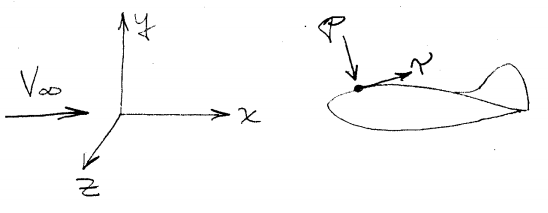
\includegraphics[width=0.5\linewidth]{Figures/p2_flowfield.PNG}
	\caption{$P$ and $\tau$ on a body in a flow field}
	\label{fig:p2_flowfield}
\end{figure}
\begin{gather*}
P = P(x,y,z)\\
\rho = \rho(x,y,z)\\
T = T(x,y,z)\\
\vec{V} = \vec{V}(x,y,z)
\end{gather*}
Knowledge of $P,\ \rho,\ T,\ \vec{V}$ as functions of x,y,z completely defines the flow field.

\subsubsection{Aerodynamic Forces}
Knowledge of $p$ and $\tau$ on the surface of a body completely defines all aerodynamic forces on the body.

\subsection{Basic Aerodynamics}
\begin{figure}[ht]
	\centering
	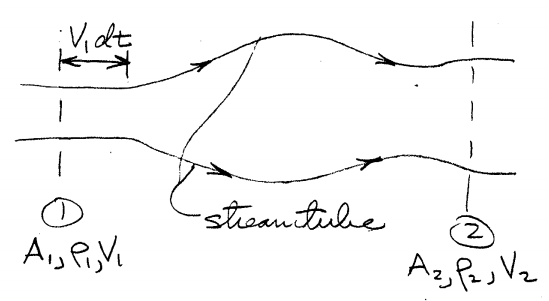
\includegraphics[width=0.5\linewidth]{Figures/p3_streamtube.PNG}
	\caption{Fluid flow in a streamtube}
	\label{fig:p3_streamtube}
\end{figure}
Continuity: conservation of mass.\\
Weight: $w = density\ \cdot volume$\\
In Figure \ref{fig:p3_streamtube}: $dw_w = \rho (V_1 dt \cdot A_1)$
\begin{gather*}
\text{Mass flow rate} = \frac{dw_1}{dt} = \dot{m_1} = \rho_1 A_1 V_1 (\frac{kg}{sec},\ \frac{slug}{sec})\\
\text{Similarly} \quad \frac{dw_2}{dt} = \rho_2 A_2 V_2
\end{gather*}
Since there can be no flow across the streamtube (by definition)
\begin{equation*}
\frac{dw_1}{dt} = \frac{dw_2}{dt} \rightarrow \boxed{\rho_1A_1V_1 = \rho_2A_2V_2}
\end{equation*}
This is the continuity equation for steady flow.

\subsection{Compressibility}
\paragraph*{} All fluids are "compressible", including water. Compressibility means that the fluid density can vary with both time and position. There are cases where a fluid can be assumed to be incompressible with good results. Flow of liquids is a common example. Also, the flow of gases such as air can also be taken as incompressible as long as the velocity remains below $\approx 225\ mph$ or $100\ m/s$.
\paragraph*{} The assumption of incompressible flow simplifies the continuity equation:
\begin{gather*}
\rho = const \rightarrow \rho_1 = \rho_2\\
V_1A_1 = V_2A_2 \quad \text{or} \quad V_2 = \big(\frac{A_1}{A_2}\big)V_1
\end{gather*}

\subsection{Momentum Equation}
\begin{figure}[ht]
	\centering
	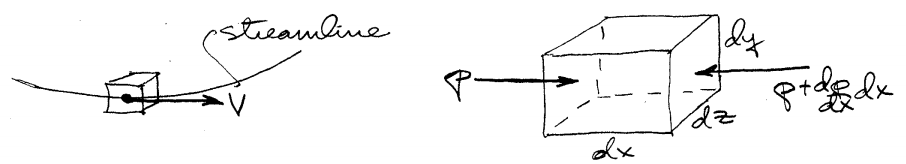
\includegraphics[width=0.8\linewidth]{Figures/p5_momentum.PNG}
	\caption{Momentum on a fluid element along a streamline}
	\label{fig:p5_momentum}
\end{figure}
Newton's Law: Force = mass $\cdot$ acceleration
\paragraph*{} Consider fluid element $dx\ dy\ dz$ moving along a streamline with velocity $V$ (Figure \ref{fig:p5_momentum}). Forces on this element include:
\begin{enumerate}
	\item pressure normal to all six faces
	\item friction tangential to all six faces
	\item gravity acting on the mass
\end{enumerate}
To begin, assume that friction and gravitational forces are negligible.
\begin{align*}
\text{Pressure force on left face} &\quad = pA = p dy\ dz\\
\text{Since pressure may vary with position}&\\
\text{Pressure force on right face} &\quad = (p + \frac{dp}{dx}dx) dy\ dz\\
\text{The force F in the x-direction is}
&\quad F=p dy\ dz - (p + \frac{dp}{dx}dx)dy\ dz\\
&\quad F = -\frac{dp}{dx}(dx\ dy\ dz)\\
\text{Mass of fluid in element} &\quad = \rho (dx\ dy\ dz)\\
\text{Acceleration of element} &\quad a = \frac{dV}{dt},\quad \text{Also } V = \frac{dx}{dt}\\
\rightarrow &\quad a = \frac{dV}{dt} = \frac{dV}{dx}\frac{dx}{dt} = \frac{dV}{dx}V\\
\text{Applying Newton's 2nd law: } F=ma &\quad -\frac{dp}{dx}(dx\ dy\ dz) = \rho(dx\ dy\ dz) V \frac{dV}{dx}\\
\rightarrow &\quad dp = \rho V dV = 0
\end{align*}
This is the momentum equation for frictionless (inviscid) flow.
\begin{figure}[ht]
	\centering
	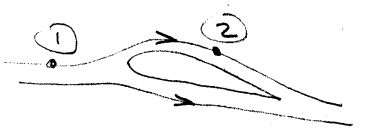
\includegraphics[width=0.3\linewidth]{Figures/p6_flowOnAirfoil.PNG}
	\caption{Flow at points 1 and 2 on an airfoil}
	\label{fig:p6_flowOnAirfoil}
\end{figure}
\paragraph*{} Consider the flow about an airfoil (Figure \ref{fig:p6_flowOnAirfoil}), and assume that it is incompressible. Integrate the momentum equation between 1 and 2.
\begin{gather*}
\int_{p_1}^{p_2} dp + \rho \int_{V1}^{V_2} V dV = 0\\p_2 - p_1 + \rho\big(\frac{V_2^2}{1}-\frac{V_1^2}{2}\big) = 0\\
p_2 + \rho\frac{V_2^2}{2} = p_1 + \rho \frac{V_1^2}{2}\\
\text{or } \boxed{p + \rho \frac{V^2}{2} = \text{const. along a streamline}}
\label{eq:Bernoulli}
\end{gather*}
which is called Bernoulli's equation. This applies only for incompressible, inviscid flows.
\paragraph*{Note:} The continuity and momentum equations relate conditions along a streamline, typically between two distinct points. The equation of state defines a relation between $\rho,\ p,\ \&\ T$ at a specific point.

\subsection{Note on Units}
\begin{align*}
\text{Dynamic Pressure} &\quad = \frac{1}{2}\rho V^2\\
\rightarrow &\quad \frac{mass}{l^3} \cdot \frac{l^2}{d^2} = \frac{F}{l^2}\\
\text{Recall }&\quad F=ma\\
\text{1 pound} &\quad = 1\ slug \cdot 1\frac{ft}{sec^2} \text{ or } 1\ slug = \frac{1\ pound}{1\ ft/sec^2}\\
\frac{1}{2}\rho V^2 &\quad = \frac{slugs}{ft^2} \cdot \frac{ft^2}{sec^2} = \frac{pound}{ft/sec^2}\cdot \frac{1}{ft^3}\cdot \frac{ft^2}{sec^2} = \frac{pound}{ft^2}\\
1\ newton = 1\ kg \cdot 1\ meter/sec^2 &\quad 1\ kg = \frac{1N}{1m/sec^2}\\
\frac{1}{2}\rho V^2 &\quad = \frac{kg}{m^3}\cdot \frac{m^2}{sec^2} = \frac{M}{m/sec^2}\cdot \frac{1}{m^3}\cdot \frac{m^2}{sec^2} = \frac{N}{m^2}
\end{align*}

\section{Applications}
\subsection{Low-Speed Wind Tunnels}
\begin{figure}[ht]
	\centering
	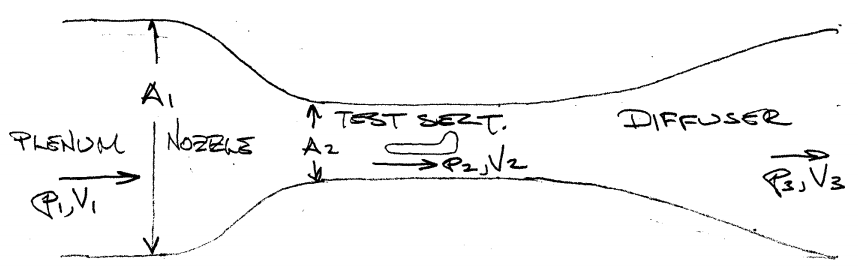
\includegraphics[width=0.7\linewidth]{Figures/p9_lowSpeedWindTunnel.PNG}
	\caption{Flow in a low-speed wind tunnel}
	\label{fig:p9_lowSpeedWindTunnel}
\end{figure}

\begin{gather*}
\text{Assume incompressible flow. Then: } \rho = const\\
\text{From continuity: } A_1V_1 = A_2V_2 \rightarrow V_2 = \big(\frac{A_1}{A_2}\big)V_1\\
\text{From Bernoulli's Equation: } p_1 + \frac{1}{2}\rho V_1^2 = p_2 + \frac{1}{2}\rho %V_2^2\\
V_1 < V_2 \rightarrow p_1 > p_2\\
\text{Solving for } V_2^2\\
V_2^2 = \frac{2}{\rho}(p_1-p_2) + V_1^2 = \frac{2}{\rho} (p_1-p_2) + \big(\frac{A_2}{A_1}\big)^2 V_2^2\\
\boxed{V_2 = \sqrt{\frac{2(p_1-p_2)}{\rho\big[ 1-(A_2/A_1)^2 \big]}}}
\end{gather*}

\subsection{Measurement of Pressure with a Manometer}
\begin{figure}[ht]
	\centering
	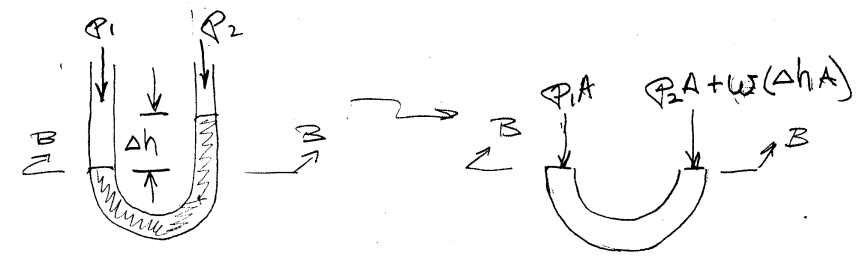
\includegraphics[width=0.7\linewidth]{Figures/p10_manometers.PNG}
	\caption{Pressure measurement using a manometer}
	\label{fig:p10_manometers}
\end{figure}
\begin{gather*}
\rho_F = \text{density of manometer fluid}\\
\text{For equilibrium} \quad p_1A = p_2A + w\Delta h A\\
\boxed{p_1-p_2 = w\Delta h = \rho_F g \Delta h}
\end{gather*}
\paragraph*{Note:} Pressures are commonly (and often most accurately) measured as "pressure differences".

% PRAGMA MARK page 11
\subsection{Measurement of Airspeed}
We desire to obtain the flow velocity by measurements at a single point. Then, we must first define "total pressure" as the pressure that would exist if the flow were slowed isentropically to zero velocity.
\paragraph*{Pitot Tube}
The pitot tube (Figure \ref{fig:p11_pitotStatic}) measures $p_0$, the total pressure. (Note there can be no flow out of the tube, therefore $V=0$.)
\paragraph*{Pitot-Static Tube}
Here, the gage measures the pressure difference $p_0-p$.

\begin{figure}[ht]
	\centering
	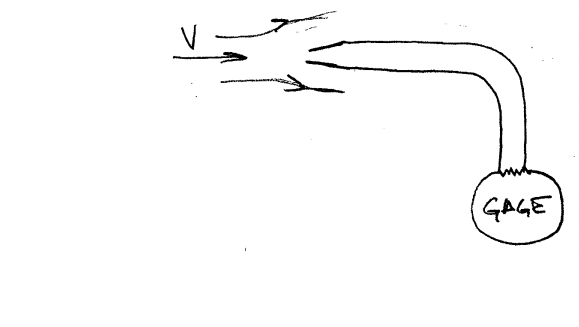
\includegraphics[width=0.4\linewidth]{Figures/p11_pitot.PNG}
	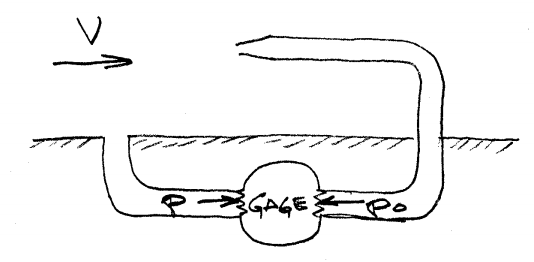
\includegraphics[width=0.4\linewidth]{Figures/p11_pitotStatic.PNG}
	\caption{Pitot (left) and pitot-static tube (right)}
	\label{fig:p11_pitotStatic}
\end{figure}

For incompressible flow, Bernoulli's Equation gives
\begin{equation*}
p + \frac{1}{2}\rho V^2 = p_0 \rightarrow \text{Static} + \text{Dynamic} = \text{Total}
\end{equation*}
From which we define "dynamic pressure" as
\begin{equation}
q = \frac{1}{2}\rho V^2
\label{eq:dynamicPressure}
\end{equation}
Bernoulli's equation can be solved for V
\begin{equation}
\boxed{V = \sqrt{2\frac{p_0-p}{\rho}}}
\label{eq:vFromBernoulli}
\end{equation}
\begin{figure}[ht]
	\centering
	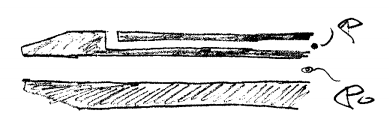
\includegraphics[width=0.4\linewidth]{Figures/p12_pitotStatic.PNG}
	\caption{Pitot-static tube}
	\label{fig:p12_pitotStatic}
\end{figure}
A pitot-static tube (Figure \ref{fig:p12_pitotStatic}) can be used to obtain the velocity at a point in the flow.
\paragraph*{Note:} You must be very careful to align the probe with the velocity vector, or the static pressure reading will be in error.
\paragraph*{} Pitot and pitot static tubes can be used to measure velocity in wind tunnels. The difficulty is in accurate measurement of static pressure (uniform flow in test section, open test section, etc.)

\subsubsection{Airplane Airspeed}
\begin{gather*}
\text{The pitot-static probe gives} \quad V_e = \sqrt{2\frac{p_0-p}{\rho_s}}\\
V_e = \text{equivalent airspeed}\\
\rho_s = \text{sea level density}\\
V_{true} = V_e \Big( \frac{\rho_s}{\rho_{actual}} \Big)^{1/2}
\end{gather*}

% PRAGMA MARK PAGE 14
\subsection{Viscous Flow}
\begin{figure}[ht]
	\centering
	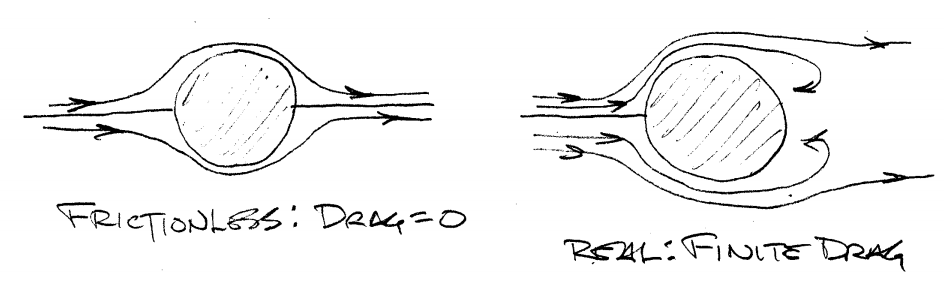
\includegraphics[width=0.8\linewidth]{Figures/p14_frictionDrag.PNG}
	\caption{Flow on a circular cylinder with real friction drag}
	\label{fig:p14_frictionDrag}
\end{figure}
Consider flow about a circular cylinder (Figure \ref{fig:p14_frictionDrag}). Frictionless flow will show zero drag about any body. This is called "d'Alembert's paradox".
\paragraph*{}In the case of a real flow, viscous effects produce drag from two primary sources:
\begin{enumerate}
	\item \textbf{Skin Friction Drag}  - a main source of drag on streamlined bodies such as wings
	\item \textbf{Separation Drag} - drag of bluff bodies such as a cylinder or a stalled wing.
\end{enumerate}

\subsection{Boundary Layer}
Thus far, analyses using Bernoulli's equation have assumed flow to have a finite, non-zero velocity at the surface of a body. In fact, there exists a very thin layer next to the body where velocity varies from a finite value to zero at the body surface. This is called the "boundary layer" (Figure \ref{fig:p15_boundaryLayer}).
\begin{figure}[ht]
	\centering
	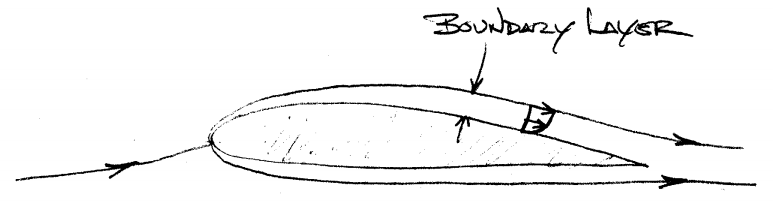
\includegraphics[width=0.5\linewidth]{Figures/p15_boundaryLayer.PNG}
	\caption{Boundary layer on an airfoil}
	\label{fig:p15_boundaryLayer}
\end{figure}
\paragraph*{} The boundary layer is a viscous phenomenon where friction between the flow and the body causes its development. Typically, for streamlined bodies, all viscous effects may be regarded as confined to this very thin layer, and the flow field outside can be calculated using the frictionless relationships such as Bernoulli's Equation.
\paragraph*{} Also, the static pressure across the boundary layer is constant. This provides a fundamental theoretical concept as introduced by Prandtl in 1906. Analysis of a flow field can be broken-up into two portions:

\begin{enumerate}
	\item The boundary layer where viscous considerations predominate.
	\item The outer region flow where frictionless analysis (potential) flow can be assumed.
\end{enumerate}

\subsubsection{Details of a Boundary Layer}
\begin{figure}[ht]
	\centering
	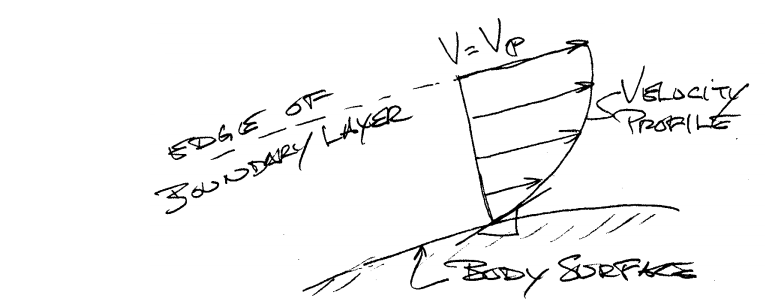
\includegraphics[width=0.6\linewidth]{Figures/p17_velocityProfile1.PNG}
	\caption{Boundary layer profile on a body surface}
	\label{fig:p17_boundaryLayer1}
\end{figure}
\begin{gather*}
\tau_w = \mu \Big( \frac{dV}{dy} \Big)_{y=0}\\
\tau_w = \text{shear stress at surface (force/unit area)}\\
\mu = \text{coefficient of viscosity}\\
\frac{dV}{dy}\Big)_{y=0} = \text{slope of velocity gradient of surface.}
\end{gather*}
\subsubsection{Laminar vs. Turbulent Boundary Layers}
\begin{gather*}
\tau = \mu \Big(\frac{dV}{dy}\Big)_{y=0}\\
\frac{dV}{dy}\Big)_{y=0,\ lam.} < \frac{dV}{dy}\Big)_{y=0,\ turb.}\\
\text{Then}\quad \tau\big)_{LAM} < \tau\big)_{TURB}
\end{gather*}
\begin{figure}[ht]
	\centering
	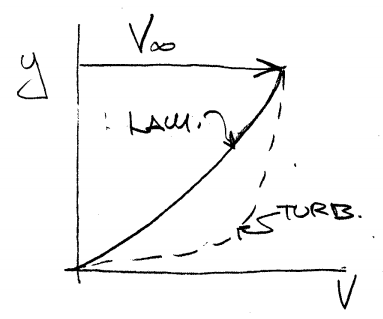
\includegraphics[width=0.3\linewidth]{Figures/p17_velocityProfile2.PNG}
	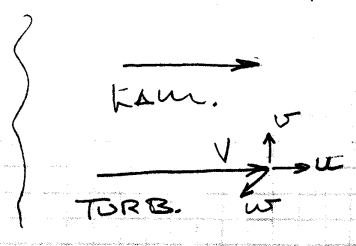
\includegraphics[width=0.3\linewidth]{Figures/p17_velocityProfile3.PNG}
	\caption{Boundary layer profile for laminar and turbulent flow}
	\label{fig:p17_boundaryLayer23}
\end{figure}

% PRAGMA MARK PAGE 18
\subsection{Reynolds Number} (similarity parameter)
\begin{gather}
RN = \frac{\rho_\infty V_\infty x}{\mu_\infty} \rightarrow \frac{\text{Inertial Forces}}{\text{Viscous Forces}}\\
x = \text{characteristic length}\\
\mu = 1.7984\cdot 10^{-5} kg/m\cdot sec = 3.7373 \cdot 10^{-7} slug/ft\cdot sec
\label{eq:Reynolds}
\end{gather}
\subsubsection{Transition}
The change in the state of a boundary layer from laminar to turbulent. Reference is often made to a "transition point", however transition actually occurs over a region of finite length which becomes significant for $RN < 10^6$.
\paragraph*{} Factors affecting transition include:
\begin{enumerate}
	\item $RN \rightarrow $ Increasing $RN$ moves transition forward.
	\item Surface roughness $\rightarrow$ increasing moves transition forward.
	\item Pressure gradient $\rightarrow dp/dx > 0 \rightarrow $ forward, $dp/dx < 0 \rightarrow$ aft.
\end{enumerate}

\subsection{Skin Friction Coefficient}
\begin{equation}
C_f = \frac{\tau_w}{\frac{1}{2}\rho_\infty V_\infty} = \frac{\tau_w}{q_\infty} = \frac{0.664}{\sqrt{RN_x}}\Big)_{LAM}
\label{eq:skinFriction}
\end{equation}
Note: $\tau =$ shear force / unit area = shear stress.\\
$q_\infty$ = normal force / unit area = pressure (dynamic).
\subsubsection{Skin Friction Drag Coefficient}
For a flat plate of length L:
\begin{equation}
D_f  = \int_0^L \tau_w dx,\quad \tau_w\big)_{LAM} = \frac{0.664}{\sqrt{RN_x}}q_\infty
\label{eq:skinFrictionDrag}
\end{equation}

\begin{gather*}
\text{Define } C_{Df} = \frac{D_f}{q_\infty L}\\C_{Df}\Big)_{LAM} = 1.328/\sqrt{RN_L},\quad \delta\Big)_{LAM} = \frac{5.2x}{\sqrt{RN_x}}\\
C_{Df}\Big)_{TURB} = 0.074/(RN)^{0.2},\quad \delta\Big)_{TURB} = \frac{0.37x}{(RN_x)^{0.2}}\\
C_{Df}\Big)_{TURB} = 0.455/(\log_{10}RN_L)^{2.58}\\
\text{where } RN_L = \frac{\rho_\infty V_\infty L}{\mu_\infty}
\end{gather*}

\subsubsection{Laminar Boundary Layer}
\begin{align*}
\delta = \frac{5.2l}{(RN_L)^{1/2}},\quad C_{fl} =& \frac{0.664}{(RN_l)^{1/2}},\quad C_f = \frac{\tau}{q_\infty}\\
D_f = \int_0^L \tau_w dx ,\quad \tau_=& \frac{0.664}{(RN_x)^{1/2}}q_\infty\\
C_{Df} = \frac{D_f}{q_\infty L}=& \frac{1}{q_\infty L}\int_0^L \tau_w dx\\
& \frac{1}{q_\infty L}\int_0^L \frac{0.664}{(RN_x)^{1/2}}q_\infty dx\\
& \frac{1}{L}\int_0^L \Big[ \frac{0.664}{(\rho_\infty V_\infty/\mu)^{1/2}}2L^{1/2} \Big]\\
C_{Df} =& \frac{1.328}{(RN_L)^{1/2}}
\end{align*}
Note: Shevell uses $C_f = C_{Df}$.

% PRAGMA MARK page 21
\subsubsection{Turbulent Boundary Layer}
See Figure \ref{fig:p21_boundaryLayer}.
\begin{gather*}
\delta = \frac{0.37l}{(RN_l)^{0.2}}\\C_{Df} = \frac{0.455}{(Log_{10}(RN_l))^{2.58}} = C_f
\end{gather*}
\begin{figure}[ht]
	\centering
	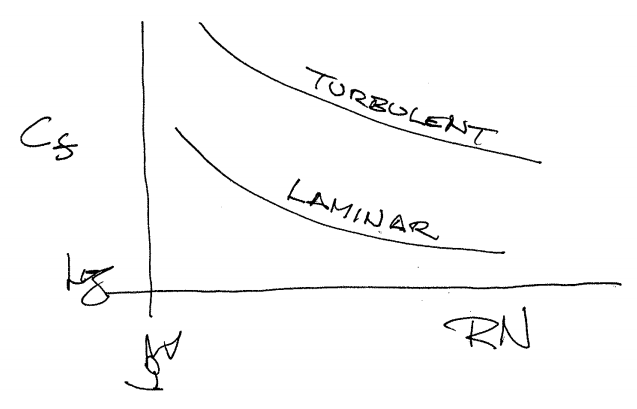
\includegraphics[width=0.5\linewidth]{Figures/p21_boundaryLayer.PNG}
	\caption{$C_f$ vs $RN$ for laminar and turbulent flow}
	\label{fig:p21_boundaryLayer}
\end{figure}

\subsubsection{Notes on Viscosity}
At sea-level on a standard day -
\begin{equation*}
\mu = 7373\cdot 10^{-7} \#\ sec/ft^2 = 1.7894 \cdot 10^{-5} kg/(m\cdot sec)
\end{equation*}
Note on units: $1 \# = 1\ slug \cdot ft/sec^2$.\\
The variation of $\mu$ with temperature is given by
\begin{gather*}
10^{10}\mu = 0.3317T^{3/2}\big( \frac{734.7}{T+216} \big)\\
\text{where}\quad T(\degree R) \text{ and } \mu(\#\ sec/ft^2)
\end{gather*}
Kinematic viscosity is defined as
\begin{equation*}
\nu = \frac{\mu}{\rho} ft^2/sec
\end{equation*}
And Reynolds number becomes
\begin{equation*}
RN = \frac{\rho vl}{\mu} = \frac{Vl}{\nu}
\end{equation*}

% PRAGMA MARK page 23
\subsection{Reynolds Number}
\begin{gather*}
RN = \frac{\rho vL}{\mu} = \frac{\rho V^2}{\mu (V/L)}\\
V/L \approx V/\delta \approx dV/dy,\quad \tau = \mu dV/dy\\
\rho V^2 = \text{ Kinetic Energy}\\
\text{Then} \quad RN = \frac{\text{Dynamic (Inertia) Forces}}{\text{Viscous Forces}} \approx \frac{\text{Pressure}}{\text{Shear}}
\end{gather*}
RN small $\rightarrow$ Viscous dominates\\
RN large $\rightarrow$ Inertia dominates.
\begin{figure}[ht]
	\centering
	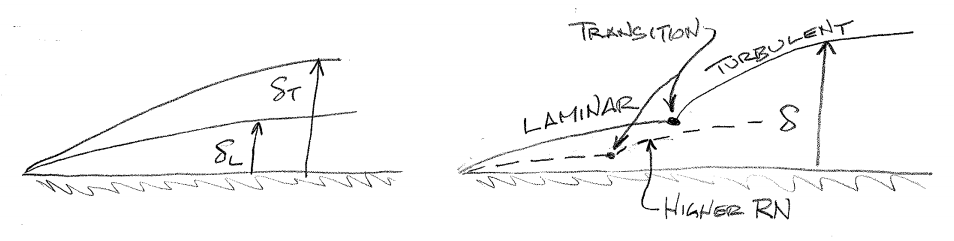
\includegraphics[width=0.8\linewidth]{Figures/p24_transitionBoundary.PNG}
	\caption{Transition between laminar and turbulent flow}
	\label{fig:p24_transitionBoundary}
\end{figure}
\begin{itemize}
\item A turbulent boundary layer is thicker than a laminar boundary layer.
\item Both laminar and turbulent boundary layers decrease in height with increase in $RN_L$.
\item Transition moves forward with increase in $RN_L$.
\end{itemize}

\begin{figure}[ht]
	\centering
	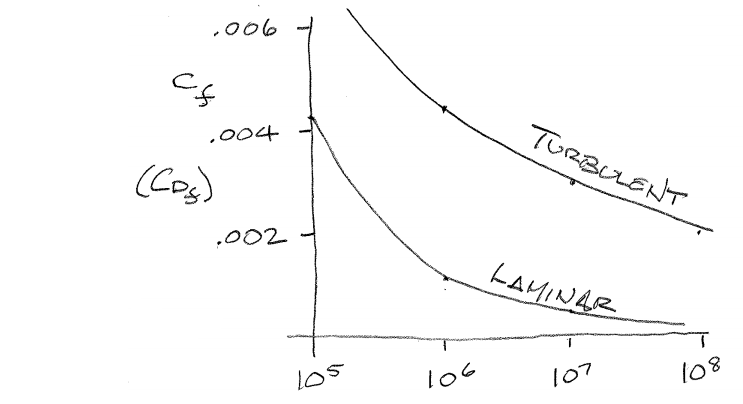
\includegraphics[width=0.6\linewidth]{Figures/p24_CdfBoundaryLayer.PNG}
	\caption{$C_{Df}$ for laminar and turbulent boundary layers}
	\label{fig:p24_CdfBoundaryLayer}
\end{figure}
\begin{equation*}
C_f = \frac{D_f}{q_\infty S_{wet}} = C_{Df}
\end{equation*}
Note: As the boundary layer develops, $\partial u / \partial y)_w$ decreases, and hence $\tau_w$ decreases.
\paragraph*{} $C_f$ is defined as the \textbf{total} smooth flat-plate skin-friction drag, i.e. the \textbf{average} over the surface from the leading edge to the trailing edge.

\subsection{Cylinder and Sphere Drag}
\begin{figure}[ht]
	\centering
	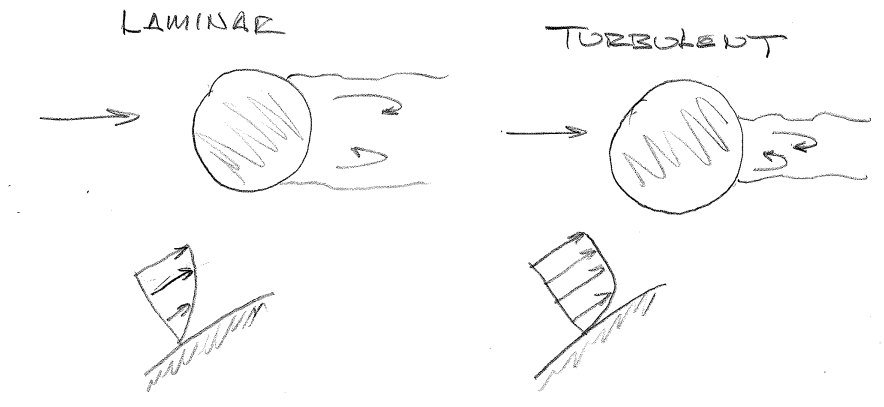
\includegraphics[width=0.7\linewidth]{Figures/p25_boundaryOnSpheres.PNG}
	\caption{Laminar and turbulent wakes on spheres}
	\label{fig:p25_boundaryOnSpheres}
\end{figure}
The turbulent boundary layer has more kinetic energy to deal with the adverse pressure gradient before separation (Figure \ref{fig:p25_boundaryOnSpheres}).
\begin{figure}[ht]
	\centering
	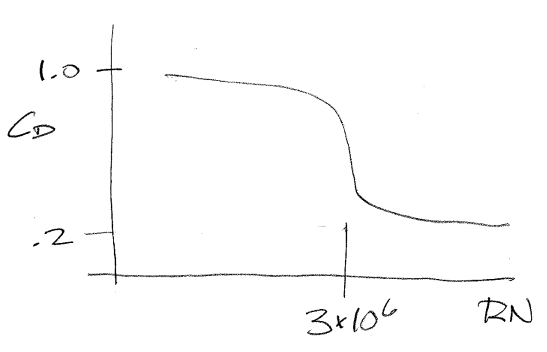
\includegraphics[width=0.4\linewidth]{Figures/p25_CdOnSphere.PNG}
	\caption{$C_D$ vs $RN$ for a spheres}
	\label{fig:p25_CdOnSphere}
\end{figure}

\subsection{Vortex Flow}
Consider the flow of a fluid in concentric circles. For equilibrium, the centrifugal force must be balanced by the pressures on the surface of the element.
\begin{figure}[ht]
	\centering
	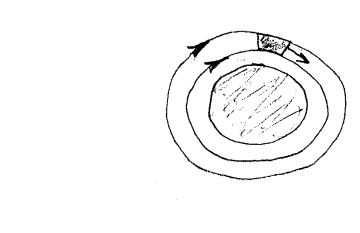
\includegraphics[width=0.3\linewidth]{Figures/p26_vortex1.PNG}
	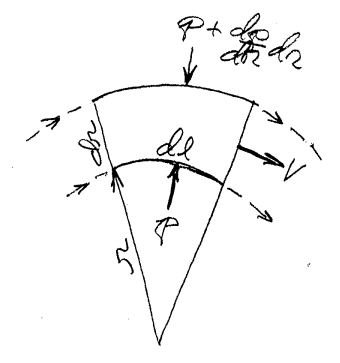
\includegraphics[width=0.25\linewidth]{Figures/p26_vortex2.PNG}
	\caption{Vortex flow}
	\label{fig:p26_vortex}
\end{figure}

\paragraph*{} Assuming unit thickness, the volume of the element is $dl/dv$, and the net pressure force acting toward the center is 
\begin{gather*}
\Big( p + \frac{dp}{dr}dr \Big) dl = pdl = \frac{dp}{dr}dr\ dl\\
% Sth illegible here
\frac{dp}{dr} = \frac{\rho V^2}{r}
\end{gather*}
Euler's equation: $dp = -\rho V dV$
\begin{gather*}
-\rho V \frac{dV}{dr} = \rho \frac{V^2}{r} \text{ or } \frac{dV}{V} = -\frac{dp}{r}
\end{gather*}
Write the Euler equation:
\begin{gather*}
dp = -\rho V\ dV \rightarrow -\rho V dV = \rho \frac{V^2}{r} dr\\
\text{Integrating} \log(V_2) = -\log(r) + const\\
\log(V_2) = const \rightarrow Vr = const \text{ or } V = \frac{const}{r} = \frac{A}{r}
\end{gather*}

Thus, the equilibrium for circular flow requires that the velocity varies as $1/r$, and this says that the velocity approaches $\infty$ as $r \rightarrow 0$.
\begin{figure}[ht]
	\centering
	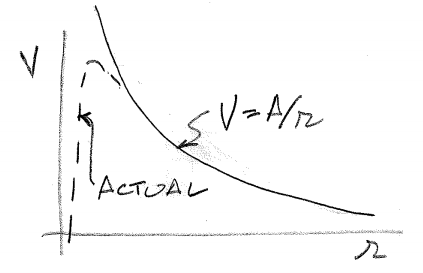
\includegraphics[width=0.3\linewidth]{Figures/p27_vortexViscousDrag1.PNG}
	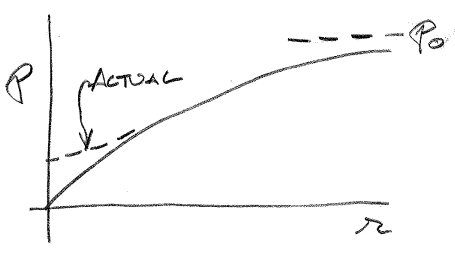
\includegraphics[width=0.3\linewidth]{Figures/p27_vortexViscousDrag2.PNG}
	\caption{Viscous drag in a vortex}
	\label{fig:vortexViscousDrag1}
\end{figure}
As the core of a vortex is approached, viscous effects begin to dominate, and the core rotates as a solid body.

% PRAGMA MARK page 28
Define $\Gamma$ as the strength of the circulatory flow.
\begin{equation*}
\Gamma = \oint \vec{V} \bullet \vec{ds} = \oint V\cos\theta ds
\end{equation*}
\begin{figure}[ht]
	\centering
	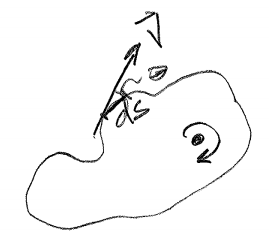
\includegraphics[width=0.25\linewidth]{Figures/p28_closedPath.PNG}
	\caption{Velocity along a closed path}
	\label{fig:p28_closedPath}
\end{figure}
$\Gamma$ is independent of path. Select a circle as the path with the vortex at the center.
\begin{equation}
\Gamma = \int_0^{2\pi} \frac{A}{r}rd\theta = 2\pi A
\end{equation}
Therefore the velocity for a vortex of strength $\Gamma$ is
\begin{equation}
V = \frac{\Gamma}{2\pi r}
\end{equation}

\paragraph*{"D'Alembert's Paradox"} For a perfect fluid (inviscid), the calculated drag of the flow about a body is zero.
\paragraph*{Superposition} A vortex can be added to the flow about a body where the resulting flow velocities are added vectorially.

\subsection{Flow About A Cylinder}
\begin{figure}[ht]
	\centering
	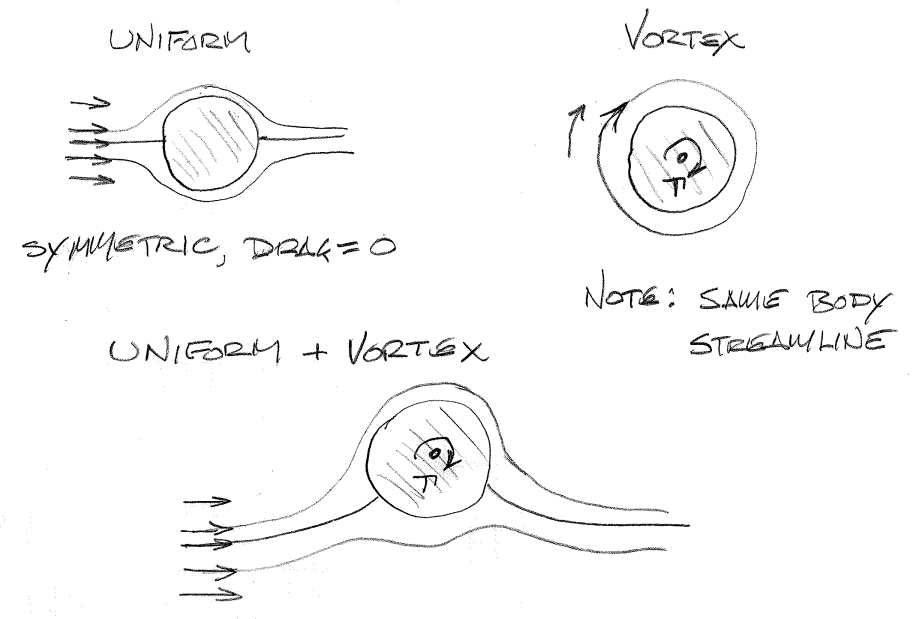
\includegraphics[width=0.8\linewidth]{Figures/p29_flowOnCylinder.PNG}
	\caption{Uniform and Vortex flow about a cylinder}
	\label{fig:p29_flowOnCylinder}
\end{figure}
Symmetric fore and aft $\rightarrow$ Drag = 0\\
Asymmetric top and bottom $\rightarrow$ Vertical Force $\neq 0$
\paragraph*{Kutta-Joukowski Law} If a circulation exists about a body in a uniform flow, a force $L$ perpendicular to the uniform flow will be produced, and $L$ is given by:
\begin{equation}
L = \rho V \Gamma
\end{equation}

% PRAGMA MARK page 30
\subsubsection{Simple Demonstration of $L=\rho V\Gamma$}
\begin{figure}[ht]
	\centering
	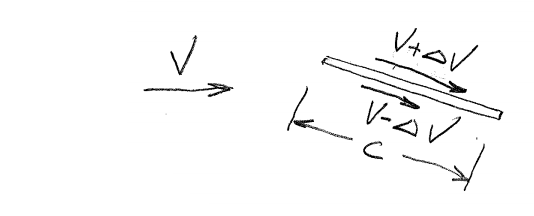
\includegraphics[width=0.4\linewidth]{Figures/p30_flatPlate.PNG}
	\caption{Flow on a flat plate}
	\label{fig:p30_flatPlate}
\end{figure}

Consider a flat plate airfoil (Figure \ref{fig:p30_flatPlate}) and assume $\Delta V$ is added to the upper surface and subtracted from the lower surface.
\begin{gather*}
p_0 = p_l + \frac{1}{2} \rho V_l^2,\quad V_l = V - \Delta V\\
p_l = p_0 - \frac{1}{2} \rho V_l^2 = p_0 - \frac{1}{2}\rho (V^2 - 2V\Delta V + \Delta V^2)\\
p_0 = p_u + \frac{1}{2} \rho V_u^2,\quad V_u = V + \Delta V\\
p_u = p_0 - \frac{1}{2}\rho V_l^2 = p_0 - \frac{1}{2}\rho (V^2 + 2V\Delta V + \Delta V^2)\\
\text{Lift} = (p_l-p_u)c = 2\rho V\Delta V_c\\
\Gamma = \oint \Delta V dx = 2\Delta V_c\\
\rightarrow \text{Lift} = \rho V\Gamma
\end{gather*}
Figure \ref{fig:p30_flowOnAirfoil} shows the flow about an airfoil.
\begin{figure}[ht]
	\centering
	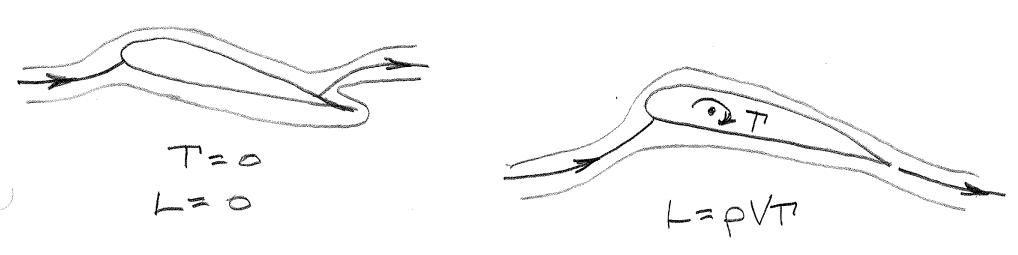
\includegraphics[width=0.8\linewidth]{Figures/p30_flowOnAirfoil.PNG}
	\caption{Flow about an airfoil}
	\label{fig:p30_flowOnAirfoil}
\end{figure}

\begin{align*}
\text{Define lift coefficient as} &\quad
C_L = \frac{L}{\frac{1}{2}\rho V^2S}\quad S = \text{Wing Area}\\
\text{Define section lift coefficient as} &\quad
C_l = \frac{L'}{\frac{1}{2}\rho V^2 c}\quad L' = \text{Lift/Unit Span}, \quad C = \text{Wing Chord}\\
\text{Then} &\quad L' = C_l \frac{1}{2}\rho V^2 c, \quad L' = \rho V\Gamma \rightarrow \Gamma = C_l \frac{Vc}{2}
\end{align*}
From theory and experiment, the lift varies linearly with angle of attack (Figure \ref{fig:p31_liftVsAOA}).
\begin{figure}[ht]
	\centering
	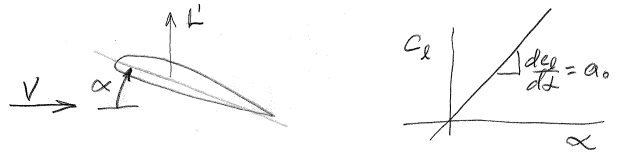
\includegraphics[width=0.8\linewidth]{Figures/p31_liftVsAOA.PNG}
	\caption{Lift varies linearly with angle of attack}
	\label{fig:p31_liftVsAOA}
\end{figure}
\begin{equation}
C_l = \frac{dC_l}{d\alpha} \alpha = a_0 \alpha
\end{equation}
($\alpha$ measured from angle where $L' = 0$.) For a perfect fluid, $a_0 = 2\pi/rad$.

% PRAGMA MARK page 32
\section{Airfoils and Wings}
\subsection{The 3-D Wing}
Helmholtz Theorems:
\begin{enumerate}
	\item A vortex filament can not end in a fluid. It extends to infinity, or forms a closed loop.
	\item The strength of a vortex filament is constant along its length.
	\item Vortices remain attached to the same fluid particles.
\end{enumerate}
\paragraph*{Prandtl's Lifting Line Theory}
\begin{figure}[ht]
	\centering
	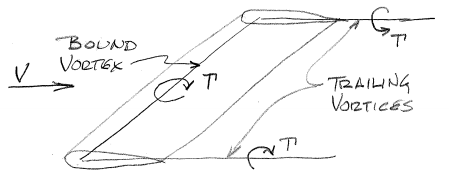
\includegraphics[width=0.6\linewidth]{Figures/p32_liftingLine.PNG}
	\caption{Bound and trailing vortices on a wing}
	\label{fig:p32_liftingLine}
\end{figure}
(Figure \ref{fig:p32_liftingLine}) Replace wing with \textbf{bound} vortex that extends downstream from each tip to form \textbf{trailing} vortices. This vortex is called a \textbf{horseshoe} vortex, and it will induce a vertical velocity behind the wing called \textbf{downwash}.

\begin{figure}[ht]
	\centering
	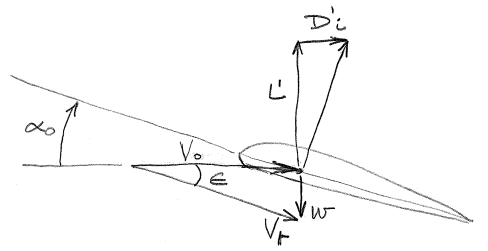
\includegraphics[width=0.6\linewidth]{Figures/p33_downwash.PNG}
	\caption{Induced downwash velocity causing induced drag}
	\label{fig:p33_downwash}
\end{figure}
The induced downwash velocity $w$ at the wing rotates the local velocity vector $V_0$ by the downwash angle $\theta$ (Figure \ref{fig:p33_downwash}). This in turn rotates the lift vector aft by the angle $\epsilon$. This creates a drag force $D_i$ parallel to $V_o$ that is called \textbf{induced drag}.
\begin{equation*}
D_i' = L' \tan\epsilon = L' \frac{w}{V_o}
\end{equation*}
The \textbf{absolute} angle of attack $\alpha_a$ is reduced by $\epsilon$ to the \textbf{effective} angle of attack $\alpha_E$.
\begin{equation*}
\alpha_E = \alpha_a-\epsilon
\end{equation*}
Induced drag is a consequence of the energy required to produce lift, and it is not caused by viscosity. The energy is spent in the trailing vortices.

\paragraph*{} A single horseshoe vortex of finite strength is inadequate to represent a finite wing. As the tip is approached the induced velocity approaches infinity, implying a negative angle of attack and hence negative lift.
\begin{figure}[ht]
	\centering
	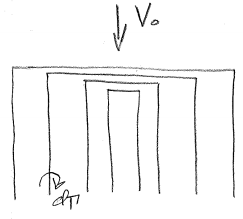
\includegraphics[width=0.25\linewidth]{Figures/p34_horseshoeVortices.PNG}
	\caption{An infinite set of horseshoe vortices representing a wing}
	\label{fig:p34_horseshoeVortices}
\end{figure}
Representing the wing with an infinite set of horseshoe vortices of strength $d\Gamma$ provides a spanwise circulation distribution that can be adjusted to meet the proper section angle of attack (and hence downwash) over the entire wing span (Figure \ref{fig:p34_horseshoeVortices}). No single horseshoe vortex has finite strength and no infinite velocities are induced.
\paragraph*{} Prandtl found that when the spanwise lift distribution varied elliptically, the induced drag, for a given lift, is a minimum. This lift distribution also results in a constant spanwise downwash.

\subsection{Characteristics of an Elliptic Spanload}
\begin{enumerate}
	\item For a wing of a given span, lift, and velocity, the drag is a minimum.
	\item The downwash is constant.
	\item An elliptic lift distribution will occur on an untwisted wing with an elliptic planform.
	\item For \#3, the value of $C_l$ will be constant along the span since $\alpha_a$ and $\epsilon$ are constant.
\end{enumerate}

\subsubsection{Shrenk Approximation}
\begin{figure}[ht]
	\centering
	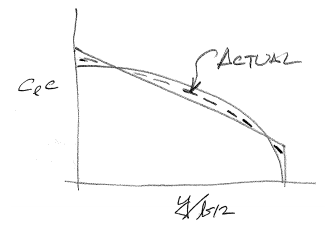
\includegraphics[width=0.4\linewidth]{Figures/p35_shrenkApproximation.PNG}
	\caption{Shrenk approximation for the lift distribution on a wing}
	\label{fig:p35_shrenkApproximation}
\end{figure}
The actual lift distance will lie halfway between the planform and an ellipse of the same area (Figure \ref{fig:p35_shrenkApproximation}). A simple tapered wing can be twisted to adjust the lift distribution to become elliptic. Again, this will result in constant downwash.
\paragraph*{} Lift distributions tend toward elliptic.

\subsection{Induced Drag}
Consider a wing with \textbf{elliptic loading}. Since the downwash is constant, the aft rotation of the lift vector is constant. Summing the section lifts and section induced drags gives:
\begin{gather*}
D_i = L\big(\frac{w}{V_o}\big) = L\epsilon\\
C_{Di} = C_L \big(\frac{w}{V_o}\big) = C_L\epsilon
\end{gather*}
\begin{align*}
\text{From Prandtl lifting line theory:} &\quad
\epsilon = \frac{C_L}{\pi AR},\quad AR = \frac{b^2}{S}\\
\text{which yields} &\quad C_{Di} = \frac{C_L^2}{\pi AR} \text{ and } \alpha_E = \alpha_a - \frac{C_L}{\pi AR} \quad \text{(Elliptic)}\\
\text{Multiplying by } \frac{1}{2}\rho V_o^2 S&\quad
\frac{1}{2}\rho V_o^2S C_{Di} = \frac{C_L^2}{\pi AR} \frac{1}{2}\rho V_o^2S = \frac{L^2}{\big(\frac{1}{2}\rho V_o^2 S\big)^2} \frac{S}{\pi b^2}\frac{1}{2} \rho V_o^2 S\\
&\quad D_i = \frac{1}{\pi q} \Big(\frac{L}{b}\Big)^2\\
\text{For non-elliptic loading}&\quad
C_{Di} = \frac{C_L^2}{\pi AR u},\quad 0.98 < u < 1.00
\end{align*}

\subsection{Lift Curve Slope of a Finite Wing}
\begin{align*}
\text{Consider a section of an elliptically loaded wing:}&\quad
\alpha_E = \alpha_a - \epsilon = \alpha_a - \frac{C_L}{\pi AR}\\
\text{And } C_L = a_o \alpha_E = a_o (\alpha_a - \frac{C_L}{\pi AR})&\quad \text{where } a_o \text{ is the 2D section lift curve slope.}\\
\text{Solving for }&\quad
C_L = \frac{a_o \alpha_a}{1+a_o/(\pi AR)}\\
\text{The 3D lift curve slope a is then}&\quad
a = \frac{dC_L}{d\alpha} = \frac{a_o}{1+a_o/(\pi AR)}\quad (\alpha \text{ in rad.})\\
&\quad a = \frac{a_o}{1+57.3a_o/(\pi AR)}\quad (\alpha \text{ in deg.})\\
\text{As AR approaches infinity, a approaches } a_o&\quad \lim_{AR\rightarrow \infty} a = a_o
\end{align*}

\subsection{Airfoils}
\begin{figure}[ht]
	\centering
	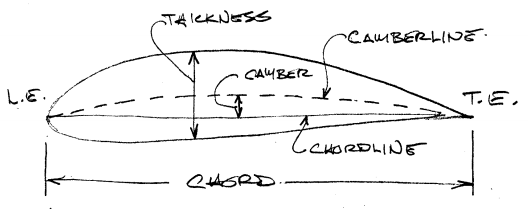
\includegraphics[width=0.5\linewidth]{Figures/p38_airfoils1.PNG}
	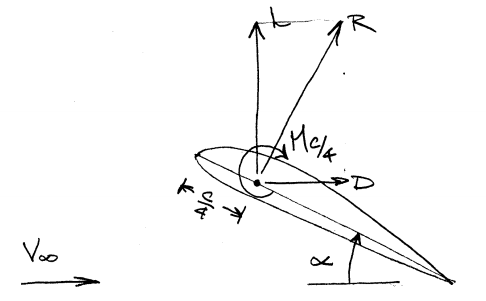
\includegraphics[width=0.4\linewidth]{Figures/p38_airfoils2.PNG}
	\caption{Airfoil parameters}
	\label{fig:p38_airfoils}
\end{figure}
An airfoil is the cross-sectional shape of a wing (Figure \ref{fig:p38_airfoils}). Typically, $M_{c/4}$ does not vary with lift coefficient. $\boxed{c/4 \approx a.c.}$

\subsection{Aerodynamic Force Coefficients}
\begin{gather*}
C_l = \frac{L}{q_\infty S} \quad \text{Lift Coefficient}\\
L (\text{Force}) = q_\infty (\text{Pressure}) \cdot S (\text{Area}) \cdot C_l (\text{Coeff.})\\
\text{Similarly} \quad C_d = \frac{D}{q_\infty S} \& C_M = \frac{M}{q_\infty Sc}
\end{gather*}
Thus, given the lift coefficient, and the flow condition $q_\infty$, the lift, drag, and moment can be calculated from:
\begin{equation}
L = C_l q_\infty S,\quad D = C_d = q_\infty S,\quad M = C_M q_\infty Sc
\end{equation}
The coefficients $C_l,\ C_d$, and $C_M$ are functions of the flow field conditions and the angle of attack, i.e.
\begin{gather*}
C_l = f_1(\alpha, M_\infty, RN)\\
C_D = f_2(\alpha, M_\infty, RN)\\
C_M = f_3(\alpha, M_\infty, RN)\\
M_\infty \text{ and } RN \text{ are "similarity parameters"}
\end{gather*}

\subsection{Airfoil Characteristics}
\begin{figure}[ht]
	\centering
	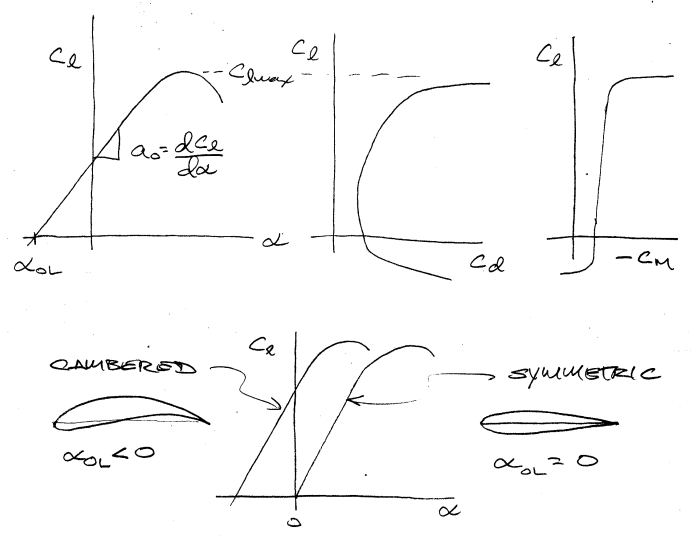
\includegraphics[width=0.7\linewidth]{Figures/p40_airfoilCharacteristics.PNG}
	\caption{Airfoil characteristics}
	\label{fig:p40_airfoilCharacteristics}
\end{figure}
Typical RN effects: Increasing RN reduces $C_d$ and increases $C_{l,max}$.\\
Subsonic $M_\infty$ effects: Increasing $M_\infty$ increases $C_d$ and reduces $C_{l,max}$.\\
Note: Apparent contradiction since:
\begin{equation*}
RN = \frac{\rho_\infty V_\infty c}{\mu_\infty},\quad M_\infty = \frac{V_\infty}{a_\infty}
\end{equation*}

\subsection{2D vs 3D Wings}
2D: Wings have infinite span. Force coefficients are defined per unit span.
\begin{equation}
C_l = \frac{L}{q_\infty c},\quad C_d = \frac{D}{q_\infty c},\quad C_m = \frac{M}{q_\infty c^2}
\label{eq:2DCoefficients}
\end{equation}
3D: Finite span.
\begin{equation}
C_L = \frac{L}{q_\infty S},\quad C_D = \frac{D}{q_\infty S},\ C_M = \frac{M}{q_\infty Sc}
\label{eq:3DCoefficients}
\end{equation}
Note: "Airfoil" refers to the 2-D "section".\\
A measure of the type of a 3-D wing is given by the "aspect ratio" (Equation \ref{eq:aspectRatio}).
\begin{equation}
AR = \frac{b^2}{S} = \frac{b^2}{bc_{rect}} = \frac{b}{c_{rect}}
\label{eq:aspectRatio}
\end{equation}

A wing with a very high aspect ratio will perform much like the airfoil section data.\\
A wing with $AR < 6$ is strongly influenced by 3-D effects, and the corresponding airfoil section data must be modified accordingly.

% PRAGMA MARK page 54a
\subsection{Stall Speed}
\begin{gather*}
C_L = \frac{L}{q_\infty S} = \frac{L}{\frac{1}{2}\rho_\infty V_\infty^2 S}\\\text{For level flight}\quad L=W\\
C_L = \frac{W}{\frac{1}{2}\rho_\infty V_\infty^2 S}\\
\text{Solving for } V_\infty \boxed{V_\infty = \Big[\frac{W}{\frac{1}{2}\rho_\infty S C_L}\Big]^{1/2}}
\end{gather*}
For a given airplane weight $W$ and wing area $S$, the lowest value of $V_\infty$ will occur when $C_L = C_{L,max}$. This lowest possible speed is called the \textbf{stall speed} (Equation \ref{eq:stallSpeed}).
\begin{equation}
V_{stall} = \Big[ \frac{W}{\frac{1}{2}\rho_\infty S C_{L,max}} \Big]^{1/2}
\label{eq:stallSpeed}
\end{equation}

\subsection{Pressure Coefficient}
\begin{equation}
C_p = \frac{p-p_\infty}{q_\infty} = \frac{p-p_\infty}{\frac{1}{2}\rho_\infty V_\infty^2}
\label{eq:CpDefinition}
\end{equation}
This definition (Equation \ref{eq:CpDefinition}) applies for \textbf{all} flows - incompressible and compressible. For incompressible flow, recall Bernoulli's equation:
\begin{gather*}
p + \frac{1}{2}\rho V^2 = p_\infty \frac{1}{2}\rho V_\infty^2\\
p - p_\infty = \frac{1}{2}\rho V_\infty^2 - \frac{1}{2}\rho V^2\\
C_p = \frac{p-p_\infty}{1/2\rho_\infty V_\infty^2} = \frac{1/2 \rho V_\infty^2 - 1/2\rho V^2}{1/2 \rho V_\infty^2}
\end{gather*}
Since for incompressible flow: $\rho = $ constant $ = \rho_\infty$
\begin{equation}
C_p = 1-\Big(\frac{V}{V_\infty}\Big)^2 \quad \text{or} \quad \frac{V}{V_\infty} = \sqrt{1-C_p}
\label{eq:CpIncompressible}
\end{equation}

\begin{figure}[ht]
	\centering
	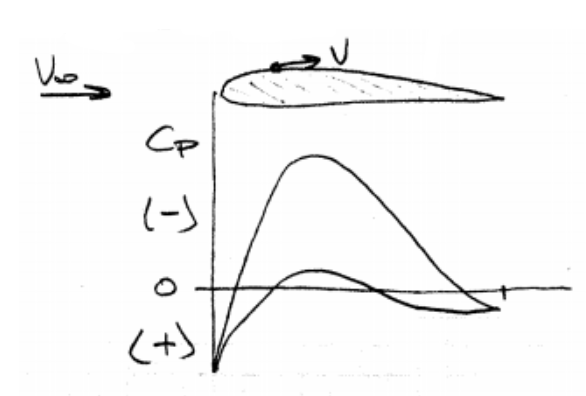
\includegraphics[width=0.4\linewidth]{Figures/p43_CpOnAirfoil.PNG}
	\caption{$C_p$ distribution on an airfoil}
	\label{fig:p43_CpOnAirfoil}
\end{figure}

As in Figure \ref{fig:p43_CpOnAirfoil}, typically, much of an airfoil's surface has $C_p$ negative. i.e. $V > V_\infty \rightarrow p < p_\infty$.

\section{Airfoils and Compressibility}
\subsection{Compressibility}
\begin{itemize}
	\item All fluids are compressible, so $\rho = \rho(x,y,z,t)$.
	\item Cases exist where density may be considered as constant and \textbf{incompressible}
	\begin{itemize}
		\item Flow of liquids
		\item Flow of gas at lower speeds
	\end{itemize}
	\item \textbf{Mach Number} is the key similarity parameter:
	\begin{equation*}
	M = \frac{\text{Flow Velocity}}{\text{Speed of Sound}} = \frac{V}{a},\quad a = \sqrt{\gamma RT}
	\end{equation*}
	\item For subsonic flight in air: $V < 225\ mph,\ M < 0.4$. The flow may be assumed incompressible. (This does not apply near $C_{L,max}$.)
	\item Compressible flow analysis requires the inclusion of the \textbf{energy equation}.\\
	The first law of thermodynamics is:
	\begin{equation*}
	de = \delta q + \delta w = \delta q - pdv
	\end{equation*}
\end{itemize}
Definitions:
\begin{enumerate}
	\item \textbf{Adiabatic Process}: No heat addition or subtraction: $\delta q = 0$
	\item \textbf{Reversible Process}: No friction or dissipation
	\item \textbf{Isentropic Process}: $\boxed{p_2/p_1 = (\rho_2/\rho_1)^\gamma}$
\end{enumerate}

\subsubsection{Speed of Sound}
\begin{figure}[ht]
	\centering
	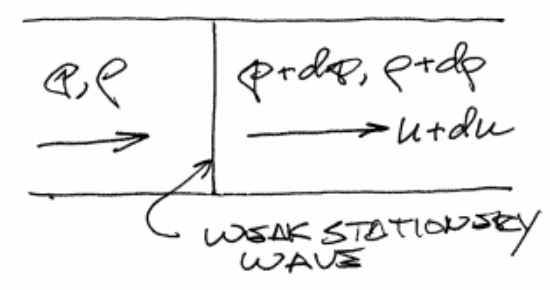
\includegraphics[width=0.4\linewidth]{Figures/p45_shockwave.PNG}
	\caption{Stationary shockwave used to derive speed of sound}
	\label{fig:p45_shockwave}
\end{figure}
\begin{align*}
\rho u &= (\rho + d\rho)(u + du) = \rho u + \rho du + u d\rho + d\rho du\\
d\rho du &\approx 0 \rightarrow u = -\rho du/d\rho\\
\text{Euler} \quad dp &= -\rho u du\\
du &= -dp/\rho u\\
u &= \frac{\rho}{dp}\frac{dp}{\rho u} = \frac{dp}{d\rho}\frac{1}{u}\\
u^2 &= \frac{dp}{d\rho}\\
\text{Assume isentropic} \quad \frac{p_2}{p_1} &= \Big(\frac{\rho_2}{\rho_1}\Big)^\gamma\\
\frac{p_2}{\rho_2} &= \frac{p_1}{\rho_1} = c\\
\rightarrow \frac{dp}{d\rho} &= \frac{d(c\rho^\gamma)}{dp} = \gamma c\rho^{\gamma-1}\\
c &= \frac{p}{\rho^\gamma} \rightarrow \frac{dp}{d\rho} = \frac{\gamma p}{\rho^\gamma}\rho^{\gamma-1} = \frac{\gamma p}{\rho}\\
u^2 &= \frac{dp}{d\rho} = \frac{\gamma p}{\rho} \rightarrow a = \sqrt{\gamma p/\rho}\\
p = \rho RT &\rightarrow \boxed{a = \sqrt{\gamma RT}}
\end{align*}

\begin{figure}[ht]
	\centering
	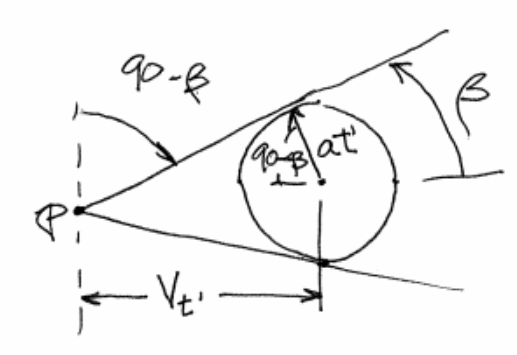
\includegraphics[width=0.4\linewidth]{Figures/p46_shockwave.PNG}
	\caption{Shockwave at angle}
	\label{fig:p46_shockwave}
\end{figure}

\begin{align*}
\sin\beta &= \frac{a t_i}{Vt_i} = \frac{a}{v} = \frac{1}{M}\\
\beta &= \arcsin\big(1/M\big)\\
\tan\beta &= \frac{at_i}{\sqrt{(Vt_i)^2 - (at_1)^2}} = \frac{1}{\sqrt{M^2-1}}\\
\beta &= \arctan\big(\frac{1}{\sqrt{M^2-1}}\big)\\
\tan(90-\beta)&= \frac{\sqrt{(Vt_1)^2-(at_1)^2}}{at_1} = \sqrt{M^2-1}
\end{align*}
\begin{figure}[ht]
	\centering
	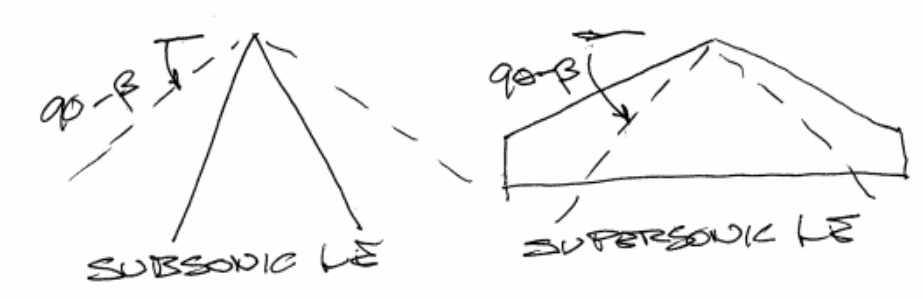
\includegraphics[width=0.7\linewidth]{Figures/p46_leadingEdge.PNG}
	\caption{Subsonic and supersonic leading edges}
	\label{fig:p46_leadingEdge}
\end{figure}

% PRAGMA MARK page 47
For incompressible flow, define $C_p$ with Equation \ref{eq:CpForLowMach}.
\begin{equation}
C_p = C_{P,0} \quad M_\infty < 0.3
\label{eq:CpForLowMach}
\end{equation}
For subsonic compressible flow, the \textbf{Prandtl-Glauer rule} gives Equation \ref{eq:PrandtlGlauerRule}.
\begin{equation}
\boxed{C_p = C_{p,0}/\sqrt{1-M_\infty^2}} \quad 0.3 < M_\infty < 0.7
\label{eq:PrandtlGlauerRule}
\end{equation}
which is a good approximation.
\begin{figure}[ht]
	\centering
	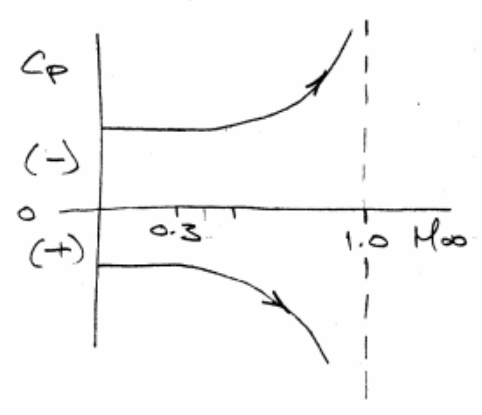
\includegraphics[width=0.4\linewidth]{Figures/p47_supersonicCp.PNG}
	\caption{$C_p$ with Prandtl-Glauer rule to account for compressibility effects}
	\label{fig:p47_supersonicCp}
\end{figure}

Note: A positive $C_p$ becomes more positive, and a negative $C_p$ becomes more negative as $M_\infty$ is increased.

\subsection{Integration of $C_p$ to Obtain Lift}
\begin{figure}[ht]
	\centering
	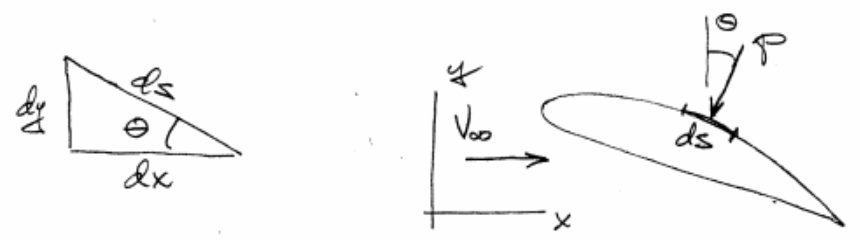
\includegraphics[width=0.7\linewidth]{Figures/p48_CpToLift.PNG}
	\caption{Integration of $C_p$ along an airfoil to obtain lift}
	\label{fig:p48_CpToLift}
\end{figure}

\begin{align*}
L &= \int_{L.E.}^{T.E.} p_l \cos\theta ds - \int_{L.E.}^{T.E.} p_u \cos\theta ds\\L &= \int_0^c p_l dx - \int_0^c p_u dx = \int_0^c (p_l-p_\infty)dx - \int_0^c(p_u-p_\infty)dx\\
\text{Define } C_l &= \frac{L}{\frac{1}{2}\rho V_\infty^2 S} = \frac{L}{q_\infty c\cdot 1} \quad \text{(unit span)}\\
	C_l &= \frac{1}{c}\int_0^c \frac{p_lp_\infty}{q_\infty}dx - \frac{1}{c}\int_0^c \frac{p_up_\infty}{q_\infty}dx\\
	C_l &= \frac{1}{2}\int_0^c(C_{pl}-C_{pu})dx\\
	\text{For compressible flow} \quad
	c_l &= \frac{1}{c} \frac{1}{\sqrt{1-M_\infty^2}}\int_0^c(C_{pl,0} - C_{pu,0})dx\\
	\boxed{C_l = C_{l,0}/\sqrt{1-M_\infty^2}} &\quad 0.3 < M_\infty < 0.7
\end{align*}

\subsection{Critical Mach No. and $C_p$}
\begin{table}
	\caption{$M_\infty$ vs $M_{peak}$}
	\centering
	\begin{tabular}{cc}
		$M_\infty$ & $M_{peak}$\\
		\hline
		0.30 & 0.43\\
		0.50 & 0.77\\
		0.61 & 1.0\\
	\end{tabular}
\end{table}
\begin{figure}[ht]
	\centering
	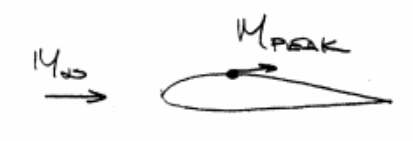
\includegraphics[width=0.4\linewidth]{Figures/p49_criticalM.PNG}
	\caption{Location of critical and peak Mach numbers on an airfoil}
	\label{fig:p49_criticalM}
\end{figure}
For a given airfoil at a given $\alpha$, as $M_\infty$ increases there is some value of $M_\infty < 1$ where $M_{peak} = 1.0$. This value of $M_\infty$ is called the "critical Mach number". When $M_\infty > M_{CR}$, there will be significant increase in drag.

\begin{figure}[ht]
	\centering
	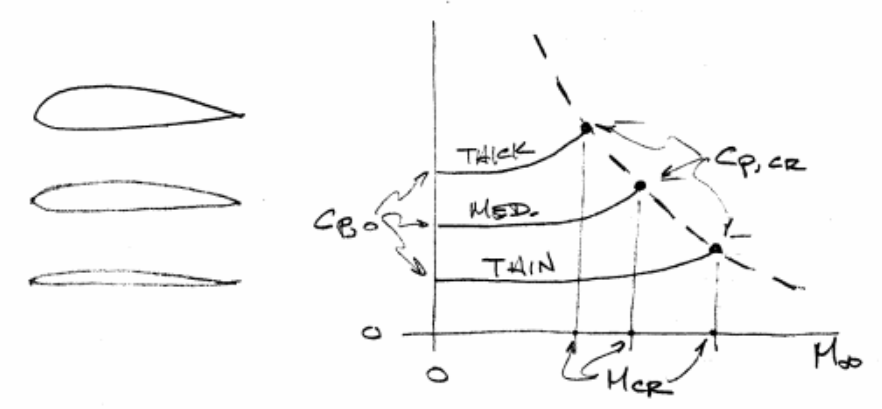
\includegraphics[width=0.8\linewidth]{Figures/p49_MVsAirfoiLThickness.PNG}
	\caption{Critical $C_p$ vs airfoil thickness}
	\label{fig:p49_MVsAirfoiLThickness}
\end{figure}

(Figure \ref{fig:p49_MVsAirfoiLThickness}) As $C_{p,0}$ at the peak becomes more negative (i.e. as the airfoil becomes thicker), $M_{CR}$ becomes lower.
\paragraph*{}The solution for the critical pressure coefficient as a function of free stream Mach number is Equation \ref{eq:CpCritical}.
\begin{equation}
C_{p,CR} = \frac{2}{\gamma M_\infty^2} \Bigg[ \Big( \frac{2+(\gamma-1)M_\infty^2}{\gamma+1} \Big)^{\gamma/(\gamma-1)} -1\Bigg]
\label{eq:CpCritical}
\end{equation}

This is universal and applies to all airfoils. For a particular airfoil, $M_{CR}$ can be determined from knowledge of the low speed value of the peak $C_o\ (C_p,0)$.
\begin{figure}[ht]
	\centering
	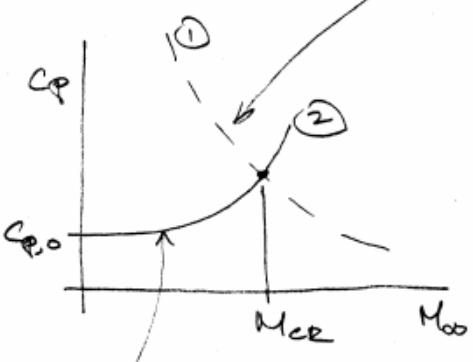
\includegraphics[width=0.4\linewidth]{Figures/p50_CpCritical.PNG}
	\caption{Critical $C_p$ and $C_{p,CR}$}
	\label{fig:p50_CpCritical}
\end{figure}
\begin{enumerate}
	\item (Figure \ref{fig:p50_CpCritical}): Plot $C_{p,CR}$ as a function of $M_\infty$.
	\item Plot $C_p$ as a function $M_\infty$ using the Prandtl-Glauer rule: $C_p = C_{p,0}/\sqrt{1-M_\infty^2}$.
	\item The integration curve (1) with (2) defines $M_{CR}$ (Figure \ref{fig:p50_CpCritical}).
\end{enumerate}

\subsection{Drag Divergence}
\begin{figure}[ht]
	\centering
	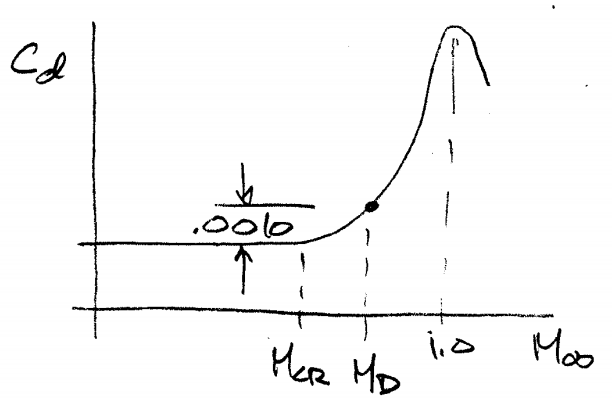
\includegraphics[width=0.5\linewidth]{Figures/p51_dragDivergence.PNG}
	\caption{Drag divergence at $M_D$}
	\label{fig:p51_dragDivergence}
\end{figure}
\begin{enumerate}
	\item For $M_\infty<M_{CR}$, the flow is subsonic ($M<1.0$) everywhere on the airfoil surface.
	\item At $M_\infty = M_{CR}$, the flow is sonic at the points of $C_{p,peak}$, and subsonic everywhere else on the airfoil surface.
	\item For $M_\infty > M_{CR}$, a supersonic region is in the neighborhood of $C_{p, peak}$, and this region is terminated by a local shock wave. The shock typically causes a substantial increase in drag. When the drag increase amounts to 0.0010, the drag divergence Mach number $M_D$ is defined (Figure \ref{fig:p51_dragDivergence}).
\end{enumerate}

\subsection{Summary of Airfoil Drag}
D = total airfoil "profile drag" = \\
\indent $D_f\ \rightarrow$ skin friction drag\\
\indent $D_p\ \rightarrow$ pressure drag\\
\indent $D_w\ \rightarrow$ wave or compressibility drag
\begin{itemize}
	\item $D_f$ due to shear forces at surface.
	\item $D_p$ due to boundary layer thickness and separation.
	\item $D_w$ due to formation of local shocks (transsonically), and bow shocks (supersonically).
\end{itemize}

% PRAGMA MARK page 53
Typical behavior of the boundary layer on an un-stalled airfoil (Figure \ref{fig:p53_boundaryOnAirfoil}).
	
\begin{figure}[ht]
	\centering
	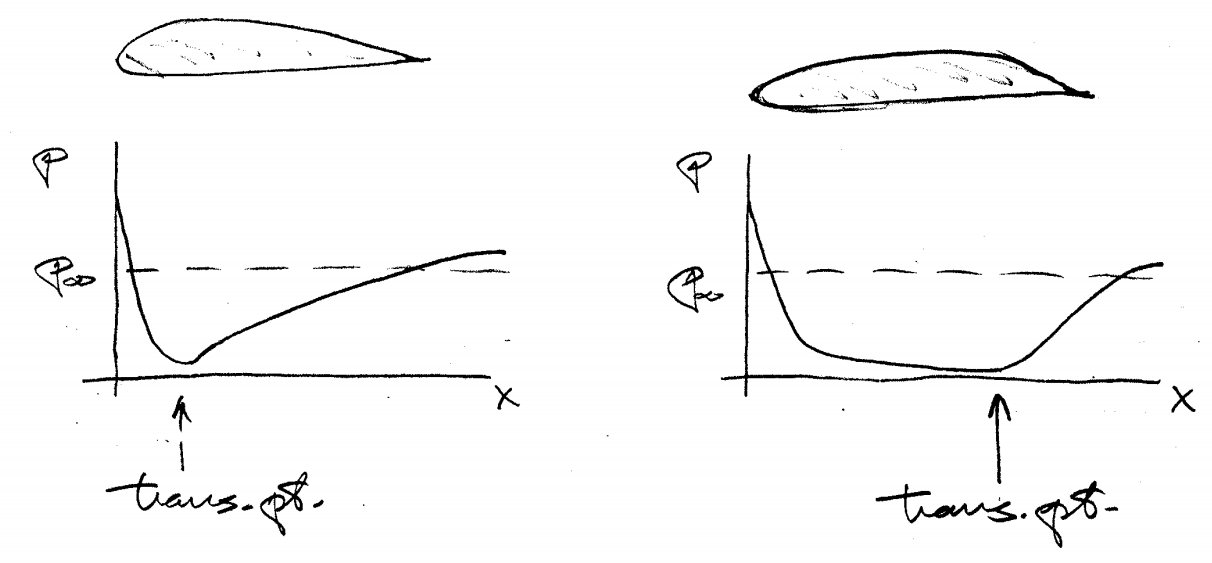
\includegraphics[width=0.8\linewidth]{Figures/p53_boundaryOnAirfoil.PNG}
	\caption{Boundary layer on a conventional and laminar flow airfoil}
	\label{fig:p53_boundaryOnAirfoil}
\end{figure}

In principle, the transition point is located further aft on the laminar airfoil, which results in lower skin friction drag. However, surface roughness can cause the transition point to move forward and the drag improvement is lost, particularly when $RN > 5\cdot 10^6$.

\subsection{Separation}
\begin{figure}[ht]
	\centering
	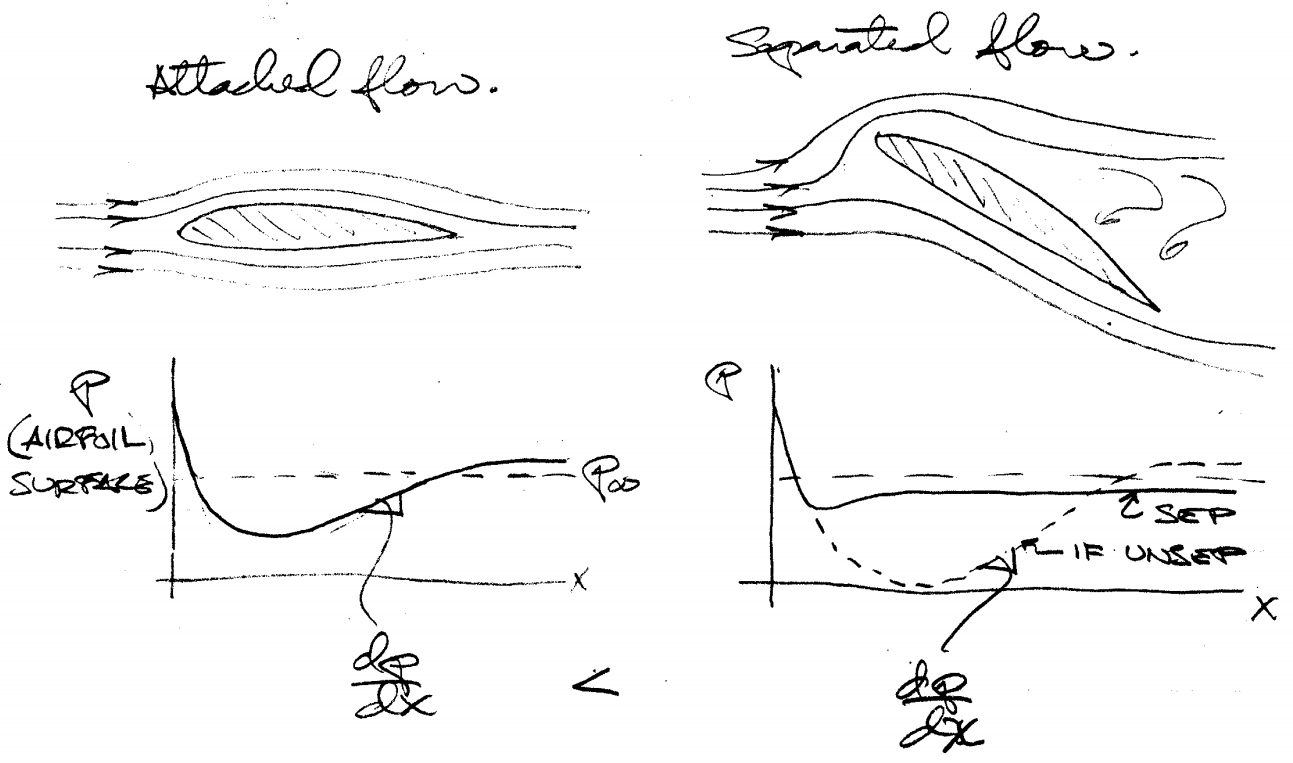
\includegraphics[width=0.9\linewidth]{Figures/p54_separationOnAirfoil.PNG}
	\caption{Attached and separated flow on an airfoil}
	\label{fig:p54_separationOnAirfoil}
\end{figure}

\begin{equation*}
\frac{dp}{dx} > 0 \rightarrow \text{"Adverse pressure gradient"}
\end{equation*}
If the required $dp/dx$ is too great, the flow will separate from the airfoil's surface (Figure \ref{fig:p54_separationOnAirfoil}).
\begin{align*}
	\text{Separation} \quad \rightarrow &\quad \text{(1) Loss of lift}\\
	&\quad \text{(2) Increase in drag}
\end{align*}
This ultimately results in the "stalling" of the airfoil.

\subsection{Drag Summary}
Two sources of drag:
\begin{enumerate}
	\item Skin friction due to shear stress at the body surface.
	\item Pressure due to flow separation. (Note: $D_p \neq 0$ even in unseparated flow.)
\end{enumerate}
\begin{gather*}
D\Big)_{total} = D_{f\ (skin\ friction)} + D_{p\ (separation)}\\
D_f\Big)_{LAM} < D_f\Big)_{TURB}
\end{gather*}
Note: High speed airplanes also experience drag due to shock waves. This is called "compressibility" or "wave" drag. It is due to a shock wave being non-isentropic.

\subsection{Compressibility Drag}
\begin{figure}[ht]
	\centering
	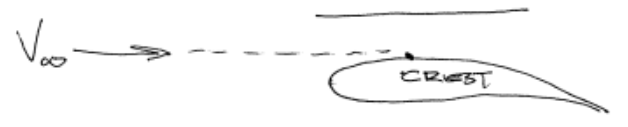
\includegraphics[width=0.6\linewidth]{Figures/p56_crest.PNG}
	\caption{Crest of airfoil}
	\label{fig:p56_crest}
\end{figure}
\begin{itemize}
\item As $M_\infty$ increases (say $M_\infty > 0.65$), local velocity on the airfoil upper surface may exceed $M=1.0$.
\item Deceleration to subsonic flow is via a shock
\begin{itemize}
	\item Drag due to reduction in $P_{total}$
	\item Drag due to boundary layer, thickening due to abrupt pressure pass.
\end{itemize}
\end{itemize}
Crest (Figure \ref{fig:p56_crest}).
\begin{itemize}
	\item Want shock ahead of crest
	\item If $M>0$ aft of crest, the supersonic flow will tend to continue to accelerate, ultimately ending with a strong shock (convergent/divergent nozzle).
\end{itemize}

\subsection{Compressibility Effect on Lift}
\begin{align*}
C_l &= \int_0^c (C_{pl} - C_{pw}) \frac{dx}{c}\\
C_p &= C_p\Big)_{INC}/\sqrt{1-M_\infty^2}\\
\rightarrow C_l &= C_l\Big)_{INC}/\sqrt{1-M_\infty^2}\\
\rightarrow C_L &= C_L\Big)_{INC}/\sqrt{1-M_\infty^2}\\
\rightarrow a,\ a_o &= a,\ a_o\Big)_{INC}/\sqrt{1-M_\infty^2} \quad \boxed{a_o = 2\pi}\text{ INC.}
\end{align*}
Define $\alpha$ = geometric angle of attack. For $\Lambda$ given $\alpha$, $C_L \ge C_L\Big)_{INC}$.

\subsubsection{Compressibility: $C_p\big)_{CRIT},\ M_{DIV}$}
\begin{gather*}
C_p = \frac{p-p_\infty}{q_\infty} = \frac{p_\infty}{q_\infty}\Big( \frac{p}{p_\infty} - 1 \Big),\quad q_\infty = \frac{\gamma}{2}p_\infty M_\infty^2\\
\frac{p_T}{p} = \Big( 1 + \frac{\gamma-1}{2}M^2 \Big)^{\gamma/(\gamma-1)},\quad \frac{p_T}{p_\infty} = \Big(1 + \frac{\gamma-1}{2}M_\infty^2\Big)^{\gamma/(\gamma-1)}\\
\frac{p}{p_\infty} = \Big( \frac{1+\frac{\gamma-1}{2}M_\infty^2}{1+\frac{\gamma-1}{2}M^2} \Big)^{\gamma/(\gamma-1)}\\
\rightarrow C_p = \frac{p_\infty}{\gamma/2p_\infty M_\infty^2}\Big[ \Big( \frac{1+\frac{\gamma-1}{2}M_\infty^2}{1+\frac{\gamma-1}{2}M^2} \Big)^{\gamma/(\gamma-1)}-1 \Big]
\end{gather*}
Define $C_p\Big)_{CRIT}$ when $M=1.0$
\begin{equation}
C_p\Big)_{CRIT} = \frac{2}{\gamma M_\infty^2} \Big[\Big( \frac{2+(\gamma-1)M_\infty^2}{\gamma+1} \Big)^{\gamma/(\gamma-1)}-1\Big]
\label{eq:CpCrit}
\end{equation}
For a given airfoil, calculate $C_p\big)_{Crest}$.
\begin{equation}
C_p\Big)_{Crest} = \frac{C_p\Big)_{INC}}{P\sqrt{1-M_\infty^2}} \quad M_{DIV} \approx 1.03 M_{CC}
\label{eq:CpvsMach}
\end{equation}
\begin{figure}[ht]
	\centering
	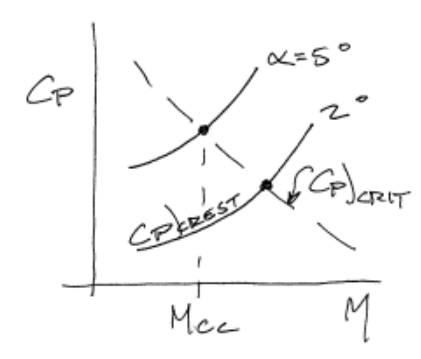
\includegraphics[width=0.4\linewidth]{Figures/p58_CpCrest.PNG}
	\caption{Crest and critical points on the M vs $C_p$ graph}
	\label{fig:p58_CpCrest}
\end{figure}

\subsection{Simple Sweep Theory}
\begin{figure}[ht]
	\centering
	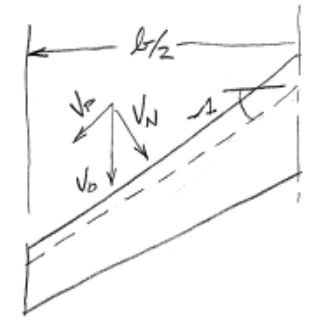
\includegraphics[width=0.3\linewidth]{Figures/p59_sweptWing.PNG}
	\caption{Swept wing}
	\label{fig:p59_sweptWing}
\end{figure}
The velocity component normal to the quarter chord line is affected by airfoil curvature, while the parallel component is not (Figure \ref{fig:p59_sweptWing}). Therefore:
\begin{align*}
V_o\Big)_{effective} &= V_o\cos\Lambda\\
M_o\Big)_{eff} &= M_o\cos\Lambda\\
q_o\Big)_{eff} = q_o\cos^2\Lambda
\end{align*}

The airfoil pressure distribution forms at the reduced mach number $M_o\cos\Gamma$. $M_{crit}$ and $M_{div}$ are increased by:
\begin{equation}
M_{crit}\Big)_\Gamma = M_{crit} \Big)_{\Lambda=0}/\cos\Lambda
\end{equation}
Also, since $q_{eff}$ is defined, to obtain the same lift:
\begin{equation}
\alpha_N = \alpha \big)_{\Lambda=0}/\cos^2\Lambda
\end{equation}
You must also consider that $t/c\Big)_N > t/c)_{\Lambda=0}$ for constant $t$. This is an effective increase in $t/c$ and a reduction in the sweep effect.

% PRAGMA MARK page 60
\subsubsection{Compressibility Effect on Wing Design}
\begin{figure}[ht]
	\centering
	\includegraphics[width=0.8\linewidth]{Figures/p60_compressibilityWingEffects.PNG}
	\caption{Effects of compressibility on wing design}
	\label{fig:p60_compressibilityWingEffects}
\end{figure}
\clearpage

\subsubsection{Classes of Airfoils}
\begin{itemize}
	\item Low speed: NACA 4415, 23012
	\item Laminar flow: NACA 64xxx
	\item High speed: Conventional, Supercritical (Figure \ref{fig:p61_AirfoilCpDistribution})
\end{itemize}

\begin{figure}[ht]
	\centering
	\includegraphics[width=0.8\linewidth]{Figures/p61_AirfoilCpDistribution.PNG}
	\caption{$C_p$ for low speed, high speed, and laminar flow airfoils}
	\label{fig:p61_AirfoilCpDistribution}
\end{figure}

Note: Both conventional and supercritical airfoils have regions of supercritical flow.
\begin{figure}[ht]
	\centering
	\includegraphics[width=0.8\linewidth]{Figures/p61_highLiftSystems.PNG}
	\caption{High-lift airfoil with slat and flap effects on $C_L$}
	\label{fig:p61_highLiftSystems}
\end{figure}
\begin{itemize}
	\item Slat increases $C_{L,max}$, but lift is constant.
	\item Flap increases lift at given $\alpha$.
	\item Typically 2 flap deflections: takeoff and landing. (Figure \ref{fig:p61_highLiftSystems})
\end{itemize}

\section{Drag}
\subsection{Total Airplane Drag}
\begin{figure}[ht]
	\centering
	\includegraphics[width=0.4\linewidth]{Figures/p62_skinFriction.PNG}
	\caption{$C_f$ vs $RN_L$ for smooth and standard roughness airfoils}
	\label{fig:p62_skinFriction}
\end{figure}

\subsubsection{Parasite Drag}
	Define "Drag area" $f$ so $f_i = K_i C_{fi} S_{wet,i}$
	\begin{itemize}
		\item $f_i$ = form factor > 1 (Accounts for thickness and sweep effects).
		\item $C_{fi}$ = skin friction coefficient (flat plate). Based on $RN_{L,i}$.
	\end{itemize}
\begin{equation}
f = \sum f_i = f_{wing} + f_{fus} + f_{tail} + f_{nac} + ...
\label{eq:dragArea}
\end{equation}
\begin{equation*}
C_{Dp} = \frac{f}{S_{ref}} \quad (S_{ref} = S_{\text{wing planform}} \text{ typically})
\end{equation*}

\begin{figure}[ht]
	\centering
	\includegraphics[width=0.8\linewidth]{Figures/p62_KWingAndTail.PNG}
	\caption{K for wing, tail, and fuselage}
	\label{fig:p62_KWingAndTail}
\end{figure}

\subsection{Drag due to Lift}
In addition to induced drag, experience has shown that a component of parasite drag increases with $C_L$. This is approximated by:
\begin{equation*}
\Delta C_{Dp} = kC_L^2
\end{equation*}
Earlier, the induced drag coefficient was given by:
\begin{equation*}
C_{Di} = \frac{C_L^2}{\pi AR u}
\end{equation*}

Where $u \approx 0.99$ is a factor to account for non-elliptic spanload. In addition, a factor S is included to account for fuselage interference.
\begin{equation}
C_{Di} = \frac{C_L^2}{\pi AR uS} \quad us \approx 0.96 - 0.98 \text{ typically}
\end{equation}
Combining the lift-dependent drag:
\begin{gather*}
C_{Di} = \frac{C_L^2}{\pi AR e} = \big( k + \frac{1}{\pi AR uS} \big) C_L^2\\
\rightarrow e = \frac{1}{\pi AR k + 1/uS} = \text{Oswald efficiency factor}\\
k = 0.38 C_{Dp} (\Lambda=0),\quad 0.40C_{Dp}(\Lambda = 20\degree),\quad 0.45 C_{Dp} (\Lambda = 35\degree)
\end{gather*}
% PRAGMA MARK page 64
\subsection{Total Incompressible Drag}
\begin{equation}
C_D = C_{Dp} + \frac{C_L^2}{\pi AR e}
\end{equation}
Solving for drag:
\begin{gather*}
D = C_D sQ = C_{Dp} sQ + \frac{C_L^2}{\pi AR e}qS\\
\text{or} \quad D = fq + \Big(\frac{L}{b}\Big)^2 \frac{1}{\pi qe}
\end{gather*}
\subsubsection{Trim Drag}
Typically, stability requires a download on the horizontal tail. This subtracts from the wing lift, and additional lift is then required.

\begin{gather*}
D_{trim} = \Big(\frac{L_w}{b}\Big)^2 \frac{1}{\pi qe} + L_H\tan\epsilon_H + \Big(\frac{L_H}{b_H}\Big)^2 \frac{1}{\pi qe_H} - \Big(\frac{L}{b}\Big)^2 \frac{1}{\pi qe}\\
D_{trim} = D_i\Big)_{wing} + D \text{ of horiz. due to } \epsilon_H + D_i\Big)_{\text{horiz.}} - D_i\Big)_{\text{No trim required}}\\
L = L_W + L_H
\end{gather*}

\section{Performance}
% PRAGMA MARK page 65
\subsection{Equations of Motion}
\begin{figure}[ht]
	\centering
	\includegraphics[width=0.6\linewidth]{Figures/p65_equationsOfMotion.PNG}
	\caption{Coordinates for aircraft equations of motion}
	\label{fig:p65_equationsOfMotion}
\end{figure}
For the general case of an airplane in flight (Figure \ref{fig:p65_equationsOfMotion}):
\begin{align*}
\sum_{\text{Parallel to F.P.}} F &= ma = m\frac{dV}{dt} = \sum F_\parallel\\
\sum_{\text{Normal to F.P.}} F &= ma = m\Big(\frac{V^2}{r_c}\Big) = \sum F_\perp
\end{align*}
\begin{enumerate}
	\item L = lift acts normal to flight path.
	\item D = drag acts parallel to flight path.
	\item W = weight acts vertically.
	\item T = thrust acts at some small angle $\alpha_T$ due to flight path.
\end{enumerate}
\begin{align*}
\sum F_\parallel &= T\cos\alpha_T - D - W\sin\theta\\
\sum F_\perp &= L + T\sin\alpha_T - W\cos\theta
\end{align*}
The general equations of motion are Equation \ref{eq:equationsOfMotion}.
\begin{align}
T\cos\alpha_T - D - W\sin\theta = m\frac{dV}{dt}\\
L + T\sin\alpha_T - W\cos\theta = m\frac{V^2}{r_c}
\label{eq:equationsOfMotion}
\end{align}

Static performance: accelerations are zero.
\begin{itemize}
	\item Level flight: $\theta = 0$
	\item Aligned thrust: $\alpha_T \approx 0$
\end{itemize}
Then, $\boxed{T=D}$ and $\boxed{L=W}$.

\subsection{Thrust Required for Level Flight}
\begin{align*}
T = D &= q_\infty S C_D\\
L = W &= q_\infty S C_L\\
\frac{T}{W} &= q_\infty S C_D/q_\infty S C_L = \frac{C_D}{C_L}\\
&\rightarrow \boxed{T_R = \frac{W}{C_L/C_D} = \frac{W}{L/D}}
\end{align*}

\begin{figure}[ht]
	\centering
	\includegraphics[width=0.4\linewidth]{Figures/p67_LDMax.PNG}
	\caption{Thrust required as a function of V}
	\label{fig:p67_LDMax}
\end{figure}

(Figure \ref{fig:p67_LDMax}) Minimum $T_R$ occurs when the aircraft is flying at $L/D\big)_{max}$.
\paragraph*{}$L/D$ is a major performance parameter relating to the "aerodynamic efficiency" of the airplane. For the $T_R$ vs $V_\infty$ curve:
\begin{enumerate}
	\item $V_\infty \rightarrow C_L = \frac{w/S}{\frac{1}{2}\rho_\infty V_\infty^2}$
	\item $C_L \rightarrow C_D = C_{Dp} + \frac{C_L^2}{\pi AR e}$
	\item $T_R = \frac{W}{C_L/C_D}$
\end{enumerate}

\begin{figure}[ht]
	\centering
	\includegraphics[width=0.8\linewidth]{Figures/p68_LDMax.PNG}
	\caption{$L/D\big)_{max}$ as a function of $C_L$ and $V_\infty$}
	\label{fig:p68_LDMax}
\end{figure}
Expanding the drag relation:
\begin{gather*}
T_R = D = q_\infty S C_D = q_\infty S \big(C_{Dp} + \frac{C_L^2}{\pi AR e}\big)\\
T_R = q_\infty S C_{Dp} + q_\infty S \frac{W^2}{q_\infty^2 S^2} \frac{1}{\pi AR e}\\
T_R = q_\infty S C_{Dp} + \frac{W^2}{q_\infty S \pi AR e}\\
T_R = \text{Parasite }T_R + \text{Induced }T_R
\end{gather*}
\begin{figure}[ht]
	\centering
	\includegraphics[width=0.5\linewidth]{Figures/p68_thrustRequired.PNG}
	\caption{$T_R$ as a function of $V_\infty$}
	\label{fig:p68_thrustRequired}
\end{figure}

Differentiate to find $T_R\big)_{max}$:
\begin{gather*}
\frac{dT_R}{dq_\infty} = S C_{Dp} - \frac{W^2}{q_\infty^2 S \pi AR e} = 0\\
\rightarrow C_{Dp} = \frac{W^2}{q_\infty^2 S^2 \pi AR e} = C_{Di}\\
\boxed{ C_{Dp}= C_{Di} \text{ for } L/D\big)_{max} \text{ and } T_{R,min} }
\end{gather*}



\subsection{Maximum $L/D$}
\begin{gather*}
C_D = C_{Dp} + \frac{C_L^2}{\pi AR e} \quad \text{(Ignore } C_{Dc})\\
\text{For } L/D\big)_{max} \rightarrow C_D/C_L \text{ is a minimum}\\
C_D/C_L = C_{Dp}/C_L + \frac{C_L}{\pi AR e}\\
\frac{d(C_D/C_L)}{dC_L} = -\frac{C_{Dp}}{C_L^2} + \frac{1}{\pi AR e} = 0\\
\end{gather*}
Substituting $C_L\big)_{L/D,max}$ yields:
\begin{gather*}
L/D\big)_{max} = \frac{(\pi C_{Dp} AR e)^{1/2}}{C_{Dp} + (\pi C_{Dp} AR e)/(\pi AR e)} =
\frac{(\pi C_{Dp} AR e)^{1/2}}{2C_{Dp}} = \frac{b}{2}\Big(\frac{\pi e}{C_{Dp}S}\Big)^{1/2}
\end{gather*}
Recalling that $C_{Dp} S = f$, the drag area:
\begin{gather*}
L/D\big)_{max} = \frac{b}{2} \Big(\frac{\pi e}{f}\Big)^{1/2}
V_{L/D,max} = \Big( \frac{2W}{\rho S C_L\big)_{L/D,max}} \Big)^{1/2} = \Big[ \frac{2W}{\rho S(\pi C_{Dp} AR e)^{1/2}} \Big]^{1/2}\\
	V_{L/D,max} = \Big[ \frac{2W}{\rho S (\pi C_{Dp} \frac{b^2}{S} e)^{1/2}} \Big]^{1/2} = \Big(\frac{2W}{\rho b}\Big)^{1/2} \Big(\frac{1}{\pi fe}\Big)^{1/4}
\end{gather*}

Solving explicitly for drag:
\begin{align*}
D &= C_D qS = C_{Dp} qS + \frac{C_L^2}{\pi AR e} qS\\
D &= fq + \frac{1}{\pi qe} \Big(\frac{L}{b}\Big)^2\\
\text{or, with } L=W \quad D &= \frac{1}{2} \rho V^2 f + \frac{1}{\pi \frac{1}{2}\rho V^2 e} \Big(\frac{W}{b}\Big)^2\\
D &= \text{Parasite} + \text{Induced}
\end{align*}

% PRAGMA MARK page 70
\begin{figure}[ht]
	\centering
	\includegraphics[width=0.4\linewidth]{Figures/p70_dragMin.PNG}
	\includegraphics[width=0.4\linewidth]{Figures/p70_dragMin2.PNG}
	\caption{Minimum drag and thrust required as a function of $V$}
	\label{fig:p70_dragMin}
\end{figure}
(Figure \ref{fig:p70_dragMin}) The variation in thrust required with speed shows the existence of:
\begin{itemize}
	\item Maximum and minimum V
	\item Several "best V's"
	\begin{itemize}
		\item Range
		\item Endurance
		\item Climb
	\end{itemize}
\end{itemize}

% PRAGMA MARK page 71
\subsection{Power Required for Level Flight}
\begin{gather*}
\text{Power} = \frac{\text{Energy}}{\text{Time}} = \frac{\text{Force}\cdot \text{Distance}}{\text{Time}} = \text{Force} \cdot \text{Velocity}\\P_r = T_r\cdot V_\infty
\end{gather*}

In terms of aerodynamic coefficients:
\begin{gather*}
C_L = \frac{W}{\frac{1}{2}\rho V_\infty^2 S} \rightarrow V_\infty = \sqrt{\frac{2W}{\rho_\infty SC_L}}\\
T_R = \frac{W}{C_L/C_D}\\
\rightarrow P_r = \frac{W}{C_L/C_D} \sqrt{\frac{2w}{\rho_\infty SC_L} = \frac{2W^3C_D^2}{\rho_\infty S C_L^3}}\\
\text{or}\quad P_R = \sqrt{\frac{2W^3}{\rho_\infty S}}\frac{1}{C_L^{3/2}//C_D}
\end{gather*}
$P_R\big)_{min}$ occurs when the aircraft is flying at $C_L^{3/2}/C_D\big)_{max}$

\begin{figure}[ht]
	\centering
	\includegraphics[width=0.5\linewidth]{Figures/p71_powerRequired.PNG}
	\caption{Power required $P_R$ vs $V_\infty$}
	\label{fig:p71_powerRequired}
\end{figure}
% PRAGMA MARK page 72
\subsubsection{Analysis of $P_R$ relation}
Expanding the $P_R$ relation:
\begin{align*}
P_R &=  DV_\infty = q_\infty S\big(C_{Dp} + \frac{C_L^2}{\pi AR e}\big) V_\infty\\P_R &= \frac{1}{2}\rho_\infty V_\infty^3 S C_{Dp} + \frac{1}{2}\rho_\infty V_\infty^3 S \frac{\Big(\frac{w}{1/2\rho_\infty V_\infty^2 S}\Big)^2}{\pi AR e}\\
\text{Parasite } P_R + \text{Induced } P_R &= \frac{1}{2}\rho_\infty V_\infty^3 S C_{Dp} + \frac{W^2}{\frac{1}{2}\rho_\infty V_\infty S \pi AR e}\\
\text{Differentiate to find } P_R\Big)_{min} &\quad \frac{dP_R}{dV_\infty} = \frac{3}{2}\rho_\infty V_\infty^2 S C_{Dp} - \frac{w^2}{\frac{1}{2}\rho V_\infty^2 S \pi AR e}\\
&= \frac{3}{2}\rho_\infty V_\infty^2S \Big[C_{Dp} - 1/3\frac{C_L^2}{\pi AR e}\Big]\\
&= \frac{3}{2}\rho_\infty V_\infty^2 S\Big(C_{Dp} - \frac{1}{3}C_{Di}\Big) = 0
\end{align*}

\begin{equation*}
\boxed{C_{Dp} = \frac{1}{3}C_{Di} \quad \text{for}\quad C+L^{3/2}/C_D\Big)_{min} \text{ and } P_R\Big)_{min}}
\end{equation*}
\begin{figure}[ht]
	\centering
	\includegraphics[width=0.5\linewidth]{Figures/p72_induced_parasite_PR.PNG}
	\caption{Power required $P_R$ vs $V_\infty$ with induced and parasite $P_R$}
	\label{fig:p72_induced_parasite_PR}
\end{figure}

The slope of a line in the $P_R$ and $V_\infty$ plane is $P_R/V_\infty$ which is equivalent to $T_R$. The minimum value of said slope (Figure \ref{fig:p73_PRMin}) occurs when the line is just tangent to the $P_R$ vs $V_\infty$ line.

\begin{figure}[ht]
	\centering
	\includegraphics[width=0.5\linewidth]{Figures/p73_PRMin.PNG}
	\caption{Slope of the $P_R$ curve at minimum power required}
	\label{fig:p73_PRMin}
\end{figure}

Solving for $C_L$ at $P_{R,min}$ yields:
\begin{align*}
C_{Dp} &= \frac{1}{3}C_{Di} = \frac{1}{3}\frac{C_L^2}{\pi AR e}\\
C_L\Big)_{PRmin} &= \big(3\pi C_{Dp} AR e\Big)^{1/2} = \sqrt{3} C_L\big)_{TRmin}\\
\text{Recalling} \quad P_R &= \Big( \frac{2W^3}{\rho_\infty S} \Big)^{1/2}\frac{1}{C_L^{3/2}/C_D}\\
\text{Substituting } C_L = C_L\big)_{min} 
P_R\Big)_{min} &= \Big(\frac{2E^3}{\rho_\infty S}\Big)^{1/2} \frac{4C_{Dp}}{\big(3\pi C_{Dp} AR e\big)}^{3/4}\\
&= \Big(\frac{2W^3}{\rho_\infty S}\Big)^{1/2} \frac{4}{(3\pi)^{3/4}}\Big[\frac{C_{Dp}}{\big(AR e\big)^3}\Big]^{1/4}\\
	&= \frac{4}{\big(3\pi\big)^{3/4}}\Big(\frac{2W^3}{\rho_\infty S} \Big)^{1/2} \Big(\frac{S}{e}\Big)^{3/4} \Big(\frac{1}{b}\Big)^{3/2} C_{Dp}^{1/4}
\end{align*}
\begin{align*}
\text{For minimum thrust} &\quad T_R\Big)_{min} = \frac{W}{L/D\big)_{max}} = \frac{2W}{\sqrt{\pi}b}\Big(\frac{S}{e}\Big)^{1/2} C_{Dp}^{1/2}\\
\text{For minimum power} &\quad P_R\Big)_{min} = \frac{2^{5/2}}{(3\pi)^{3/4}}
\Big(\frac{1}{\rho_\infty}\Big)^{1/2} S^{1/4} \Big(\frac{1}{e}\Big)^{3/4} \Big(\frac{W}{b}\Big)^{3/2}C_{Dp}^{1/4}
\end{align*}

\subsection{Power Available}
\begin{equation*}
\text{Reciprocating prop: } P_A = \eta P \quad \text{Turbojet: } T_A \approx const\cdot  V_\infty\quad P_A = T_A V_\infty \rightarrow \text{linear}
\end{equation*}
In Figure \ref{fig:p75_PA}, the jet power is linear. Then, speed = efficiency.
 
 \begin{figure}[ht]
 	\centering
 	\includegraphics[width=0.3\linewidth]{Figures/p75_PAprop.PNG}
 	\includegraphics[width=0.3\linewidth]{Figures/p75_PAjet.PNG}
 	\caption{Power available vs $V_\infty$ for a propeller (left) and jet (right)}
 	\label{fig:p75_PA}
 \end{figure}

\subsubsection{Maximum Speed}
 \begin{figure}[ht]
	\centering
	\includegraphics[width=0.8\linewidth]{Figures/p75_maxSpeed}
	\caption{Power vs maximum speed for a propeller (left) and jet (right)}
	\label{fig:p75_maxSpeed}
\end{figure}

$V_{max}$ and $V_{min}$ are set by the intersections of the $P_A$ and $P_R$ curves.
\paragraph*{Note:} Operating below $V_{min}$ results in $P_R>P_A$, and hence the expression "backside of the power curve".

\subsubsection{Altitude Effects on $P_R$}
Recall the expressions
\begin{equation}
V = \sqrt{\frac{2w/s}{\rho C_L}},\quad P_R = \sqrt{\frac{2w^2C_D^2}{\rho S C_L^3}}
\end{equation}
Note that for a given $C_L$, both $V$ and $P_R$ are proportional to $1/\rho^{1/2}$. Therefore, denoting sea level conditions by the subscript $\big)_o$
\begin{gather*}
V_{alt} = V_o \Big(\frac{\rho_o}{\rho}\Big)^{1/2}\\
P_{R,alt} = P_{R,o}\Big(\frac{\rho_o}{\rho}\Big)^{1/2} \quad\rightarrow\quad C_L = const.
\end{gather*}
For now assume:
\begin{equation}
P_{A,alt} = P_{A,o}\Big(\frac{\rho_o}{\rho}\Big) \quad \text{and}\quad T_{A,alt} = T_{A,o} \Big(\frac{\rho}{\rho_o}\Big)
\end{equation}
Note: Both $P_R$ and $V$ shift due to changes in $\dot{m}$ aft. $V$ shifts due to maintaining $C_L =$ const.
 \begin{figure}[ht]
	\centering
	\includegraphics[width=0.5\linewidth]{Figures/p76_PowerAltitude}
	\caption{Power vs altitude}
	\label{fig:p76_PowerAltitude}
\end{figure}

\subsection{Rate of Climb}
 \begin{figure}[ht]
	\centering
	\includegraphics[width=0.8\linewidth]{Figures/p77_rateOfClimb}
	\caption{Rate of climb and flight path angle}
	\label{fig:p77_rateOfClimb}
\end{figure}
For equilibrium:
\begin{gather}
T = D = W\sin\theta \quad (\parallel \text{ flight path})\\
L = W\cos\theta \quad (\perp \text{ flight path})
\end{gather}
\begin{gather*}
\text{Multiply by } V_\infty \quad TV_\infty = DV_\infty + WV_\infty\sin\theta\\
\boxed{R/C = V_\infty \sin\theta = \frac{TV_\infty - DV_\infty}{W}}\\
R/C = \frac{\text{Excess Power}}{W} \quad (\theta < 20^\degree)
\end{gather*}
 \begin{figure}[ht]
	\centering
	\includegraphics[width=0.7\linewidth]{Figures/p77_excessPower}
	\caption{Excess power vs $V_\infty$ for a prop and jet}
	\label{fig:p77_excessPower}
\end{figure}

% PRAGMA MARK PAGE 78
\paragraph*{Note:} For a given $V_\infty$, the lift required is actually $L=W\cos\theta$, and hence $C_L$ is reduced as $\theta$ increases. Consequently the power required in climb is reduced as $\theta$ increases. For $\theta < 20^\degree$ this is negligible.

\subsubsection{Maximum Rate and Angle of Climb}
Note: In Figure \ref{fig:p78_maxRateAngleofClimb}, $V_{max,\theta} < V_{max,R/C}$.
 \begin{figure}[ht]
	\centering
	\includegraphics[width=0.7\linewidth]{Figures/p78_maxRateAngleofClimb}
	\caption{Maximum rate and angle of climb for prop and jet aircraft}
	\label{fig:p78_maxRateAngleofClimb}
\end{figure}

% PRAGMA MARK page 79
\subsubsection{Climb Speeds}
 \begin{figure}[ht]
	\centering
	\includegraphics[width=0.3\linewidth]{Figures/p79_climbSpeedVInfty}
	\caption{Rate of climb}
	\label{fig:p79_climbSpeedVInfty}
\end{figure}
\begin{gather}
R/C = \frac{T-D}{W}V\\
\text{Gradient} = \frac{R/C}{V_\infty} = \frac{T-D}{W}
\end{gather}
Max R/C speeds, prop: $P_A \approx $ const. w/r/t/ V.
\begin{gather*}
R/C = \frac{P_A-P_R}{W} \quad P_R\big)_{min} \rightarrow R/C \big)_{max}\\
V_{R/C,max} = \Big(\frac{W/S}{1/2 \rho C_{L,Pin}}\Big)^{1/2} \quad C_{L,Pin} = \big(3 \pi C_{Dp} AR e\big)^{1/2}
\end{gather*}
\textbf{Jet} $T_A \approx$ const. w/r/t V.
\begin{gather*}
V_{R/C)_{max}}\Big|_{jet} > V_{R/C)_{max}}\Big|_{prop} \quad \text{for the same }P_R
\end{gather*}

\begin{figure}[ht]
	\centering
	\includegraphics[width=0.3\linewidth]{Figures/p79_Prprop}
	\includegraphics[width=0.3\linewidth]{Figures/p79_Prjet}
	\caption{Power required $P_R$ and available $P_A$ for a prop (left) and jet (right)}
	\label{fig:p79_Pr}
\end{figure}
\textbf{Max Gradient Speeds}:
\begin{equation*}
Grad = \frac{t}{W} - \frac{1}{L/D} \quad L/D\big)_{max} \rightarrow \text{ Max Grad}
\end{equation*}
\textbf{Min Fuel Speeds}: Increasing speed over $V_{R/C,max}$ will increase range with a minor decrease in R/C.
\begin{equation*}
V_{econ} > V_{R/C,max}
\end{equation*}

% PRAGMA MARK page 80
\paragraph*{Note on Climb Speeds}
\begin{equation}
\text{Prop:} \quad R/C = \frac{P_A-P_R}{W},\quad \text{Grad} = \frac{R/C}{V}
\end{equation}
For $P_A =$ const, maximum R/C is obtained at $C_L^{3/2}/C_D\big)_{max}$. Maximum grad will be obtained at $V < V_{R/C,max}$.

\begin{equation}
\text{Jet:} \quad  R/C = \Big( \frac{T}{W} - \frac{1}{L/D} \Big)V \quad \text{Grad} = \frac{T}{W} - \frac{1}{L/D}.
\end{equation}
For $T_A =$ const, maximum grad is obtained at $C_L/C_D\big)_{max}$. Maximum R/C will be obtained at $V > V_{L/D,max}$.\\
Note: $V_{C_L/C_D,max} > V_{C_L^{3/2}/C_D,max}$ for prop and jet.

% PRAGMA MARK page 81
\subsection{Ceilings}
Consider the power curves at sea level and some altitude.\\
In Figure \ref{fig:p81_ceiling} $P_R$ changes by altitude. See altitude effects on $P_A$ and $P_R$.
\begin{figure}[ht]
	\centering
	\includegraphics[width=0.4\linewidth]{Figures/p81_ceiling.PNG}
	\caption{Power vs $V_\infty$ curve at sea level (solid line) and altitude (dashed line)}
	\label{fig:p81_ceiling}
\end{figure}
Finally, there is some altitude where $P_R = P_A$ at a single point, and $P_R > P_A$ everywhere else. This altitude is the "absolute ceiling". The "service ceiling" (Figure \ref{fig:p81_serviceCeiling}) is where $R/C\big)_{max} = 100\ ft/sec$, and this is a practical upper limit.
\begin{figure}[ht]
	\centering
	\includegraphics[width=0.3\linewidth]{Figures/p81_ceilingPower.PNG}
	\includegraphics[width=0.3\linewidth]{Figures/p81_serviceCeiling.PNG}
	\caption{(Left): Power required and available for absolute ceiling. (Right): Service ceiling}
	\label{fig:p81_serviceCeiling}
\end{figure}
\clearpage

\subsection{Time to Climb}
\begin{gather*}
R/C = \frac{dh}{dt} \quad \text{(a vertical velocity)}\\
dt = \frac{dh}{dh/dt} = \frac{dh}{R/C}\\
\text{time}\ \Big|_{h_1}^{h_2} = \int_{h_1}^{h_2}\frac{dh}{R/C}\\
\text{time}\ \Big|_{\text{Sea Level}}^{h} = \int_0^h \frac{dh}{R/C}
\end{gather*}

To solve for time to climb, calculate the $R/C$ for several different altitudes and plot $(R/C)^{-1}$ vs $h$. The area under the curve is the time to climb (Figure \ref{fig:p82_timeToClimb}).
\begin{figure}[ht]
	\centering
	\includegraphics[width=0.5\linewidth]{Figures/p82_timeToClimb.PNG}
	\caption{Time to climb as area under the $(R/C)^{-1}$ curve}
	\label{fig:p82_timeToClimb}
\end{figure}

\subsection{Range}
\begin{align*}
\text{Specific range = miles / \# fuel} &= \frac{\text{Miles/hr}}{\text{\# fuel/hr}} = \frac{V}{CT} = \frac{V}{CD}\\
\text{For a jet:} \quad C&= \frac{\text{\# fuel}}{\text{\# thrust/hr}} = SFC\\
\text{For a jet: specific range} &= \frac{V}{C}L/D \frac{1}{W}\\
\text{For a prop:}\quad  C &= \frac{\text{\# fuel}}{\text{BHP/hr}}\\
\text{For a prop: specific range} &= \frac{V}{C\cdot \text{BHP}} = \frac{V}{C\cdot \text{THP}/\eta}\\
\text{For a prop:} &= const \cdot \frac{\eta}{C}L/D \frac{1}{W}\quad const = 325( \text{knots, HP, \#})
\end{align*}
\paragraph*{Jet:} for max SR, $V$ should be slightly greater than $V_{L/D,max}$. Also, $V_{L/D,max}$ increases with altitude.\\
\textbf{Prop:} Max SR is independent of altitude. Increasing altitude increases $V_{L/D,max}$.\\
\textbf{Both:} Increasing altitude increases $V_{L/D,max}$. $C_L$ is slightly less than $C_L\big)_{L/D,max}$ for \textbf{speed stability}.

\begin{equation*}
\text{Range} = \int \frac{\text{Miles}}{\text{\# fuel}} dW
\end{equation*}
Assuming average (const.) values for $\eta,\ C,\ L/D$:
\begin{align*}
\text{Jet:}\quad R_J &= \int_{W_f}^{W_i} \frac{V}{C}L/D \frac{dW}{W} = \frac{V}{C} L/D\log_e\big(\frac{W_i}{W_f}\big)\ \text{(NMI)}\\
\text{Prop:} \quad R_P &= \int_{W_f}^{W_i} 325 \frac{\eta}{C} L/D\frac{dW}{W}= 325 \frac{\eta}{C}L/D \log_e\big(\frac{W_i}{W_f}\big)\ \text{(NMI)}\\
const\ L/D \rightarrow\ const\ C_L \rightarrow\ \text{cruise climb}
\end{align*}
\begin{figure}[ht]
	\centering
	\includegraphics[width=0.5\linewidth]{Figures/p84_range.PNG}
	\caption{Payload vs range}
	\label{fig:p84_range}
\end{figure}
Editor Note: in Figure \ref{fig:p84_range}, $P/L$ is a shorthand for payload. Range is given in nautical miles (NMI).
\begin{figure}[ht]
	\centering
	\includegraphics[width=0.9\linewidth]{Figures/p84_flightPlan.PNG}
	\caption{Flight plan with altitude}
	\label{fig:p84_flightPlan}
\end{figure}

% PRAGMA MARK page 85
For a jet, maximum range will occur at $V_{C_L/C_D,max}$, \textbf{neglecting compressibility drag}.
\begin{gather*}
V = \Big(\frac{2W/S}{\rho C_L}\Big)^{1/2}\\
V_{C_L/C_D,max} = \Big(\frac{2W/S}{\rho C_L}\Big)^{1/2} \cdot \frac{C_L}{C_D} = \Big(\frac{2W/S}{\rho}\Big)^{1/2}\frac{C_L^{1/2}}{C_D}\quad
\text{then max range }\rightarrow\ \frac{C_D}{C_L^{1/2}}\Big)_{min}\\
\frac{C_D}{C_L^{1/2}} = \frac{C_{Dp}}{C_L^{1/2}} + \frac{C_L^{3/2}}{\pi AR e}\\
\frac{d}{dC_L} \Big(\frac{C_D}{C_L^{1/2}}\Big) = -\frac{1}{2}\frac{C_{Dp}}{C_L^{3/2}} + \frac{3C_L^{1/2}}{2\pi AR e} = 0\quad \text{then} 
\rightarrow C_{Dp} = 3\frac{C_L^2}{\pi AR e}\\
C_L\Big)_{max\ R} = \frac{1}{3^{1/2}} (C_{Dp}\pi AR e)^{1/2} = \frac{1}{3^{1/2}}C_L\Big)_{L/D,max}\\
\frac{V_{max\ R}}{V_{L/D,max}} = \Big[\frac{C_L\big)_{L/D,max}}{C_L\big)_{max\ R}}\Big]^{1/2} = 3^{1/4} = 1.32
\end{gather*}
With compressibility drag constraining speed, best range is obtained by increasing altitude at $M$ = const until drag is a minimum (approaching $L/D_{max}$).

% PRAGMA MARK page 86
\subsection{Endurance}
Specific endurance = hours / \# fuel.
\begin{align}
\text{Jet} &= \frac{1}{TC} = \frac{1}{CD} = \frac{L}{CDW}\\
\text{Prop} &= \frac{1}{\text{BHP}C} = \frac{1}{C\cdot\text{THP}/\eta} = \frac{\eta }{CVW}L/D
\end{align}
Endurance is the integral:
\begin{align*}
E_{jet} &= \int_{W_f}^{W_i} \frac{1}{C}\frac{L}{D}\frac{dW}{W} = \frac{L}{CD} \log_e \Big(\frac{W_i}{W_f}\Big)\\
\text{Note:} &\quad E_{jet} V = R_{jet},\quad \text{fly at } L/D\big)_{max}\\
E_{prop} &= \int_{W_f}^{W_i} \frac{\eta}{C} \frac{L}{D} \frac{1}{V} \frac{dW}{W},\quad V = \Big(\frac{2W/S}{\rho C_L}\Big)^{1/2}\\
 &= \int_{W_f}^{W_i} \frac{\eta}{C} \Big(\frac{\rho S}{2}\Big) \frac{C_L^{3/2}}{C_D} \frac{dW}{W^{3/2}}\\
E_{prop} &= 2\frac{\eta}{C} \Big(\frac{\rho S}{2}\Big)^{1/2} \frac{C_L^{3/2}}{C_D} \Big(\frac{1}{W_f^{1/2}} - \frac{1}{W_i^{1/2}}\Big)
\end{align*}
Fly at minimum altitude and $C_L^{3/2}/C_D\big)_{max}$.

\subsubsection{Range and Endurance (prop)}
Reciprocating engines are rated in terms of
\begin{equation}
\text{SFC} = \frac{\text{\# fuel}}{\text{BHP}\cdot hr}
\end{equation}
For maximum \textbf{endurance}, \# fuel/hr must be minimized:
\begin{equation*}
\frac{\text{\# fuel}}{AR} = \text{SFC} \cdot P_{req}
\end{equation*}
For maximum endurance: $P_{req}\big)_{min} \rightarrow \frac{C_L^{3/2}}{C_D}\big)_{max}$.
\paragraph*{}\noindent For maximum \textbf{range}, \# fuel /mile must be minimized:
\begin{equation*}
\frac{\text{\# fuel}}{\text{mile}} = \text{SFC} \cdot P_{req}\cdot \frac{hr}{mile} = \frac{\text{SFC}\cdot P_{req}}{V_\infty} = \text{SFC} \cdot T_{req}
\end{equation*}
Max range occurs when $T_{req}\big)_{min} \rightarrow \frac{C_L}{C_D}\big)_{max}$ (Figure \ref{fig:p87_maxRange}).
\begin{figure}[ht]
	\centering
	\includegraphics[width=0.4\linewidth]{Figures/p87_maxRange.PNG}
	\caption{Maximum range occurs when required thrust is minimized.}
	\label{fig:p87_maxRange}
\end{figure}

% PRAGMA MARK page 88
Let C = SFC $= \frac{\text{\# fuel}}{\text{BHP}\cdot hr}$.
\begin{align*}
C\cdot P \cdot dt &= \text{\# fuel used in dt}\\
&= \text{changing W of airplane in time increment dt}\\
W_o &= \text{TOGW}\\
W_i &= \text{weight of airplane without fuel}\\
W_i &= W_o - W_f\\
dW\big)_{airplane} &= dW_f = -cP\ dt
\end{align*}
(Minus sign due to weight decreasing as time is increasing.)

\begin{equation}
E = \int_0^E dt = -\int_{W_o}^{W_i} \frac{dW}{cP}, \quad \text{and } dt = -\frac{dW}{cP}
\end{equation}
Similarly, for range:
\begin{gather*}
ds = V_\infty dt = -\frac{V_\infty dw}{cP}\\
R = \int_0^R ds = -\int_{W_o}^{W_i} \frac{V_\infty dw}{cP}
\end{gather*}

Note on units:
\begin{align*}
\frac{1}{C} = \frac{\text{BHP}\cdot hr}{\#} &= 550 \frac{ft\#}{sec} \cdot \frac{3600\ sec}{hr}\cdot \frac{hr}{\#}\\
&= 550 \cdot 3600\ ft\\
&= 550 \cdot \frac{3600}{5280}\ \text{miles}
\end{align*}
\hrule

\begin{gather*}
\frac{\rho_\infty S}{W} = \frac{slug}{ft^2} \cdot \frac{ft^2}{\#} = \frac{slug}{ft \cdot \#}\\
1\# = 1\ slug \cdot \frac{ft}{sec^2} \rightarrow slug = \frac{\#\ sec^2}{ft}\\
\frac{\rho_\infty S}{W} = \frac{slug}{ft \#} = \frac{1}{ft \#}\cdot \frac{\#\ sec^2}{ft} = \Big(\frac{sec}{ft}\Big)^2\\
\frac{1}{C} \Big(\frac{\rho_\infty S}{W}\Big)^{1/2} = 550\cdot 3600\ ft \big(\frac{sec}{ft}\big) = 550\cdot 3600\ sec = 550\ hr
\end{gather*}

\subsection{Breguet Equations (Prop)}
For steady, level flight:
\begin{align*}
P &= \frac{P_{req}}{\eta} = \frac{DV_\infty}{\eta}\\R &= \int_{W_i}^{W_o}\frac{V_\infty\ dw}{CP} = \int_{W_i}^{W_o} \frac{V_\infty \eta\ dw}{C D V_\infty} = \int_{W_i}^{W_o} \frac{\eta\ dw}{CD}\\
R &= \int_{W_i}^{W_o} \frac{\eta W}{CD} \frac{dW}{W} = \int_{W_i}^{W_o} \frac{\eta L}{CD} \frac{dW}{W}
\end{align*}
In general, $\eta,\ C$, and $L/D$ can be assumed to remain constant during a flight.
\begin{gather*}
\rightarrow R = \frac{\eta L}{CD} \int_{W_i}^{W_o} \frac{dW}{W} = \frac{\eta L}{CD} \Big(\log W_o - \log W_1\Big)\\
\boxed{R = \frac{\eta L}{CD} \log \Big( \frac{W_o}{W_i} \Big)}
\end{gather*}
For max R: $\eta$ should be high and $c$ low.
\begin{equation*}
W-o/W_i = \frac{W_i + W_f}{W_i} = 1 + \frac{W_f}{W_i}\ \text{high} \rightarrow \text{fly at } L/D\Big)_{max}
\end{equation*}

% PRAGMA MARK page 91
\begin{align*}
E &= \int_{W_i}^{W_o} \frac{dW}{CP} = \int_{W_1i}^{W_o} \frac{\eta}{C} \frac{dW}{DV_\infty} = \int_{W_i}^{W_o} \frac{\eta L}{CD V_\infty} \frac{dW}{W}\\
V_\infty &= \Big[\frac{2W}{\rho_\infty S C_L}\Big]^{1/2}\\
E &= \int_{W_i}^{W_o} \frac{\eta}{C} \frac{C_L}{C_D} \Big(\frac{\rho_\infty S C_L}{2}\Big)^{1/2} \frac{dW}{W^{3/2}}
\end{align*}
If $C_L,\ C_D,\ \eta,\ C$ are assumed constant:
\begin{equation*}
\boxed{E = 2\frac{\eta}{C} \frac{C_L^{3/2}}{C_D} \Big(\frac{\rho_\infty S}{2}\Big)^{1/2} \Big(\frac{1}{W_i^{1/2}} - \frac{1}{W_o^{1/2}}\Big)}
\end{equation*}

Max E: Same as max R except:
\begin{enumerate}
	\item Fly at $C_L^{3/2}/C_D\Big)_{max}$.
	\item Fly at $\rho = \rho_{max} =$ sea level.
\end{enumerate}

\subsubsection{Range and Endurance (Jet)}
Turbojet engines are rated by:
\begin{equation*}
\text{TSFC} = \frac{\text{\# fuel}}{\text{\# thrust}\cdot hr}
\end{equation*}
where it should be noted that TSFC is not dimensionless. For maximum \textbf{endurance:} $\frac{\text{\# fuel}}{hr} =$ TSFC $\cdot T$.\\
Maximum endurance is $T_{req}\Big)_{min} \rightarrow \frac{C_L}{C_D}\Big)_{max}$.
\paragraph*{} For maximum range:
\begin{gather*}
\frac{\text{\# fuel}}{mile} = \frac{\text{TSFC}\cdot T}{V_\infty}\\
\frac{T}{V_\infty} = \frac{D}{V_\infty} = \frac{\frac{1}{2} \rho_\infty V_\infty^2 S C_D}{V_\infty} = \frac{1}{2} \rho_\infty V_\infty S C_D\\
V_\infty = \Big(\frac{2W}{\rho_\infty C_L S}\Big)^{1/2}\\
\frac{T}{V_\infty} = \frac{1}{2}\rho_\infty S \Big(\frac{2W}{\rho_\infty C_L S}\Big)^{1/2} \quad
C_D = \Big(\frac{\rho_\infty WS}{2}\Big)^{1/2} \frac{1}{C_L^{1/2}/C_D}
\end{gather*}
For maximum range: $\frac{T}{V_\infty}\Big)_{min} \rightarrow \frac{C_L^{1/2}}{C_D}\Big)_{max}$.

% PRAGMA MARK page 93
\noindent Let $C_t = $ TSFC $= \frac{\text{\# fuel}}{\text{\# thrust}\cdot hr}$.
\begin{align*}
C_t \cdot T \cdot dt &= -dW\\
dT &= -\frac{dW}{CT}\\
E = \int_0^Edt &= -\int_{W_o}^{W_i} \frac{dW}{C_t T} = \int_{W_i}^{W_o} \frac{L}{C_t D}\frac{dW}{W}
\end{align*}
Assuming $C_t$ and $C_L/C_D$ are constant over the duration of the flight:
\begin{equation}
\boxed{E = \frac{1}{C_t}\frac{C_L}{C_D}\log \Big( \frac{W_o}{W_i} \Big)}
\end{equation}
Max E: $C_t$ low and $W_o/W_1 = 1 + W_f/W_1$ high. Fly at $L/D\big)_{max}$.
\paragraph*{Note:} This result is very similar to the condition for maximum range of a propeller-driven aircraft.

% PRAGMA MARK page 94
\noindent For the range of a turbojet airplane:
\begin{gather*}
ds = V_\infty\ dt = -\frac{V_\infty\ dW}{C_t T}\\
R = \int_o^R ds = -\int_{W_o}^{W_i} \frac{V_\infty\ dW}{C_t T}
\end{gather*}

\begin{align*}
\text{Recalling that }T = W/(C_L/C_D) &\quad
R = \int_{W_i}^{W_o}\frac{V_\infty C_L}{C_t C_D}\frac{dW}{W}\\
\text{and using} &\quad V_\infty = \Big(\frac{2W}{\rho_\infty C_L S}\Big)^{1/2}\\
&\quad R = \int_{W_i}^{W_o} \Big(
\frac{2}{\rho_\infty S}\Big)^{1/2}\frac{C_L^{1/2}/C_D}{C_t} \frac{dW}{W^{1/2}}
\end{align*}
Assuming $C_t,\ C_L,\ C_D$ are constant:
\begin{equation}
\boxed{R = \Big(\frac{8}{\rho_\infty S}\Big)^{1/2} \frac{C_L^{1/2}}{C_t C_D} \Big( W_o^{1/2} - W_i^{1/2} \Big)}
\end{equation}
Max R: $C_t$ low, $W_f$ high. Fly at $C_L^{1/2}/C_D\big)_{max}$ and $\rho_\infty\big)_{min}$ (for high altitude) to maximize range.

\subsection{Range}
\begin{align}
SR\big)_{jet} &= \frac{V}{C} L/D \frac{1}{W}\\
SR\big)_{prop} &= 325\frac{\eta}{C}L/D \frac{1}{W}
\end{align}
\textbf{Assume $C_L$ = const}
\begin{align*}
R\big){jet} &= \int_{W_f}^{W_i} \frac{V}{C} L/D \frac{dW}{W} = \frac{V}{C} L/D \log \Big(\frac{W_i}{W_f}\Big)\\
&\rightarrow V = const \rightarrow \rho \text{ varies}\\
V &= \Big(\frac{2W}{\rho C_L S}\Big)^{1/2}\\
R\big)_{jet} &= \int_{W_f}^{W_i} \Big(\frac{2}{\rho S}\Big)^{1/2} \frac{C_L^{1/2}/C_D}{C} \frac{dW}{W^{1/2}}\\
&= \Big(\frac{8}{\rho S}\Big)^{1/2} \frac{1}{C} C_L^{1/2}/C_D \big(W_i^{1/2} - W_f^{1/2}\big)\\
&\rightarrow \rho = const \rightarrow V \text{ varies}
\end{align*}

\begin{align*}
R\big)_{prop} &= \int_{w_f}^{w_i} 325 \frac{\eta}{C} C_L/C_D \frac{dW}{W} = 325 \frac{\eta}{C} C_L/C_D \log\Big(\frac{w_i}{w_f}\Big)\\
&\rightarrow \rho \text{ and } V \text{ vary to maintain } C_L = const\\
\frac{C_L}{C_D}\Big)_{max} &\rightarrow C_L = \big(\pi AR e C_{Dp}\big)^{1/2}\\
\frac{C_L^{1/2}}{C_D}\Big)_{max} &\rightarrow C_L = \big(\frac{1}{3} \pi AR e C_{Dp}\big)^{1/2}
\end{align*}

% PRAGMA MARK page 96
\subsection{Endurance}
\begin{align}
SE\big)_{jet} &= \frac{1}{C} L/D \frac{1}{W}\\
SE\big)_{prop} &= \frac{\eta}{C} L/D \frac{1}{WV}
\end{align}
\textbf{Assume $C_L$ = const.}
\begin{align*}
E\big)_{jet} &= \int_{w_f}^{w_i} \frac{1}{C} C_L/C_D \frac{dW}{W} = \frac{1}{C} C_L/C_D \log\Big(\frac{w_i}{w_f}\Big)\\
&\rightarrow \rho \text{ and } V \text{ vary to maintain } C_L = const
\end{align*}
\begin{align*}
E\big)_{prop} &= \int_{w_f}^{w_i} \frac{\eta}{CV} C_L/C_D \frac{dW}{W},\quad V = \Big(\frac{2W}{\rho C_L S}\Big)^{1/2}\\
&= \int_{w_f}^{w_i} \frac{\eta}{C} \Big(\frac{\rho S}{2}\Big)^{1/2} C_L^{3/2}/C_D \Big(\frac{1}{w_f^{1/2}} - \frac{1}{w_i^{1/2}}\Big)\\
&\rightarrow \rho = const \rightarrow V \text{ varies}\\
\frac{C_L^{3/2}}{C_D}\Big)_{max} &\rightarrow C_L = \big(3\pi AR e C_{Dp}\big)^{1/2}
\end{align*}

% PRAGMA MARK page 97
\section{Applications}
\subsection{Takeoff}
\begin{align*}
a &= \frac{F}{m} = \frac{T-D}{W/g} = \frac{T-C_DqS-\mu(W-L)}{W/g}\\
a &= \frac{ T - \big[ C_{Dp} qS + K_L \frac{C_{L}t^2}{\pi AR e} + \mu (W-C_{Lt}qS) \big] }{W/g}
\end{align*}
Where:
\begin{itemize}
	\item $C_{Lt}$ = taxi $C_L$, $K_L$ = ground effect $< 1$
	\item $\mu$ = rolling coefficient = 0.15 for hard surfaces or 0.50 for grass
	\item $C_{Dp}$ includes flaps and landing gear
\end{itemize}
Distance from brake release to liftoff:
\begin{gather*}
d_{Lo} = \int_0^{t_{Lo}} at\ dt = \frac{at^2_{Lo}}{2} \quad \text{IF a is constant}\\
V_{Lo} = at_{Lo} \rightarrow d_{Lo} = \frac{V_{Lo}^2}{2a}
\end{gather*}

$T$ and $D$ in fact vary with $V$, however, an \textbf{effective average} value for $T-D$ is that when $V=\frac{1}{\sqrt{2}}V_{Lo} = 0.707 V_{Lo}$, this yields $d_{Lo} = V_{Lo}^2/(2a_{0.7V_{Lo}})$.\\
Using $V_{Lo} = 1.2 V_{stall}$:
\begin{equation}
V_{Lo} = 1.2 \Big(\frac{2W/S}{\rho C_{L,max}\big)_{T/O}}\Big)^{1/2}
\end{equation}

% PRAGMA MARK page 98
This yields for $d_{Lo}$:
\begin{align*}
d_{Lo} &= 1.44 \frac{2W/S}{\rho C_{L,max}\big)_{T/O}}\frac{1}{2\Big( \frac{T-D}{W/g} \Big)_{0.7V_{Lo}}}\\
&= 1.44 \frac{W^2}{ g\rho SC_{L,max}\big)_{T/O} \big(T-D\big)_{0.7V_{Lo}} }
\end{align*}
During takeoff, $D<<T$ and using $T=\rho/\rho_o$:
\begin{equation*}
d_{Lo} = f\Big(\frac{W^2}{ \sigma S C_{L,max}\big)_{T/O} T_{0.7V_{Lo}} }\Big)
\end{equation*}
which is often written as
\begin{equation*}
K = \frac{W}{S} \frac{W}{T_{0.7V_{Lo}}} \frac{1}{\sigma C_{L,max}\big)_{T/O}}
\end{equation*}
$W/S$ = wing loading, $W/T$ = thrust loading.
\paragraph*{Ground run} is typically 80\% of the total distance to clear $35\ ft$ height. Therefore, $K$ is a good parameter to correlate TOFL (Figure \ref{fig:p98_KParameter}).

\begin{figure}[ht]
	\centering
	\includegraphics[width=0.5\linewidth]{Figures/p98_KParameter.PNG}
	\caption{K with all engines operating}
	\label{fig:p98_KParameter}
\end{figure}
\begin{figure}[ht]
	\centering
	\includegraphics[width=0.9\linewidth]{Figures/p99_takeoff.PNG}
	\caption{Schematic of takeoff forces}
	\label{fig:p99_takeoff}
\end{figure}

Assuming $F$ is constant:
\begin{equation*}
F = ma = m\frac{dV}{dt} \rightarrow t = \frac{Vm}{F} \rightarrow S = \frac{V^2 m}{2F}
\end{equation*}
In general:
\begin{gather*}
F = T-D-R = T-D-\mu_r(W-L)\\
L = \frac{1}{2}\rho_\infty V_\infty^2 S C_L\\
D = \frac{1}{2} \rho_\infty V_\infty^2 S \big(C_{Do} + \frac{C_L^2}{\pi AR e}\big)\\
\text{Assuming } F \approx const \text{ and } V_{Lo} = 1.2V_s = 1.2\sqrt{\frac{W}{\frac{1}{2}\rho_\infty S C_{L,max}}}\\
S_{Lo} = \frac{1.44 W^2}{ g\rho_\infty S C_{L,max} \big[ T-D-\mu_r (W-L)_{avg} \big] }
\end{gather*}
For \textbf{landing}, set $T=0$ or $T<0$.

\begin{figure}[ht]
	\centering
	\includegraphics[width=0.8\linewidth]{Figures/p100_fieldLength.PNG}
	\caption{Balanced field length}
	\label{fig:p100_fieldLength}
\end{figure}

\subsection{Landing Field Length}
\begin{figure}[ht]
	\centering
	\includegraphics[width=0.8\linewidth]{Figures/p101_landing.PNG}
	\caption{Landing field length}
	\label{fig:p101_landing}
\end{figure}
Definitions for Figure \ref{fig:p101_landing}.
\begin{align*}
L &= W\cos\gamma\\
D_{ef} &= D-T = W\sin\gamma\\
L/D &= \frac{1}{\tan\gamma} = \frac{d_{gl}}{50}\\
d_{dec} &= \frac{V^2_{50}}{2a} - \frac{V_L^2}{2a},\quad D_{ef} = \frac{W}{q}a,\quad L\approx W\\
\rightarrow d_{dec} &= \frac{1}{2} \frac{W}{q} \Big(V_{50}^2 - V_L^2\Big)/D_{ef}
\end{align*}
\begin{align*}
d_{air} &= d_{gl} + d_{dec} = \frac{L}{D_{ef}} \Big[50 + \frac{1}{2q} \Big( V_{50}^2 - V_L^2 \Big)\Big]\\
d_g &= \frac{V_L^2}{2a} = \frac{1}{2}\frac{WV_L^2}{qR},\quad R=D+\mu\big(W-L\big)
\end{align*}
Since $V_{50}$ and $V_L$ are both $\approx V_S^2$:
\begin{equation*}
d_{land} = d_{air} + d_G = A + BV_S^2
\end{equation*}
\begin{figure}[ht]
	\centering
	\includegraphics[width=0.4\linewidth]{Figures/p101_farFl.PNG}
	\caption{Far FL = $d_{land}/0.6$}
	\label{fig:p101_farFl}
\end{figure}
See Figure \ref{fig:p101_farFl}.

% PRAGMA MARK page 102
\begin{figure}[ht]
	\centering
	\includegraphics[width=0.8\linewidth]{Figures/p102_landing.PNG}
	\caption{Landing field length without air deceleration}
	\label{fig:p102_landing}
\end{figure}
In Figure \ref{fig:p102_landing}:
\begin{equation*}
C_{L,max} = \frac{296W/S}{\sigma V_s^2}
\end{equation*}
F.A.R.'s require $V_{50} = 1.3V_s$ and $V_{td} = 1.15V_s$. Landing field length = $S_T/0.6$.\\
Energy equation: K.E. + P.E. = Drag $\cdot$ Distance.
\begin{gather*}
W\frac{V_{50}^2-V_{td}^2}{2g} + 50W = D\cdot S_{50}\\
S_{50} = \frac{L}{D} \Big[ \Big( \frac{V_{50}^2-V_{td}^2}{2g} \Big) + 50 \Big] = \frac{L}{D} \big(0.0162V_s^2 + 50\big)
\end{gather*}
Assume ground deceleration = $-a$ (less reversers).
\begin{gather*}
S_g = V_{td}^2/(-2a) = -1.88V_s^2/a\\
V_s^2 = \frac{296W/S}{\sigma C_{L,max}},\quad S_f = \big(S_{50}+S_g\big)/0.6\\
\boxed{ S_f = \frac{L}{D} \Big( \frac{8W/S}{\sigma C_{L,max}} + 83.3 \Big) + \frac{925W/S}{-a\sigma C_{L,max}}}
\end{gather*}
From this equation we see high $C_{L,max}$ and low $L/D$ are desirable.

% PRAGMA MARK page 103
\subsection{Stability and Control}
Equilibrium: $\sum F = \sum M = 0$.
\paragraph*{Static Stability:} Forces and moments on a body caused by a disturbance tend initially to return the body towards equilibrium (Figure \ref{fig:p103_stability}).

\begin{figure}[ht]
	\centering
	\includegraphics[width=0.8\linewidth]{Figures/p103_stability.PNG}
	\caption{Static stability example}
	\label{fig:p103_stability}
\end{figure}
\paragraph*{Dynamic Stability:} After a disturbance, a body, out of its own accord, returns to equilibrium over a period of time (Figure \ref{fig:p103_dynamicStability}).
\begin{figure}[ht]
	\centering
	\includegraphics[width=0.8\linewidth]{Figures/p103_dynamicStability.PNG}
	\caption{Response for dynamically stable and unstable systems}
	\label{fig:p103_dynamicStability}
\end{figure}

\paragraph*{Control}
\begin{enumerate}
	\item Change from one equilibrium position to another.
	\item Produce non-equilibrium accelerations.
\end{enumerate}
\paragraph*{Moments:}
\begin{enumerate}
	\item Recall that at the aerodynamic center, $C_m$ is constant with respect to $C_L$.
	\item At $C_L=0$, there are no force vectors, and $C_m$ is the result of a pure couple which is invariant with respect to position on the body.
	\item Therefore, at $C_L=0$:
	\begin{equation*}
	C_{mac} = C_{mac}\big)_{C_L=0} = C_{m,any\ pt.}\big)_{C_L=0}
	\end{equation*}
\end{enumerate}

\begin{figure}[ht]
	\centering
	\includegraphics[width=0.6\linewidth]{Figures/p104_aircraftStability.PNG}
	\caption{Force and moment balance on an aircraft with CG and $M_{ac}$.}
	\label{fig:p104_aircraftStability}
\end{figure}
	An airplane (Figure \ref{fig:p104_aircraftStability}) is said to be \textbf{trimmed} if:
	\begin{equation}
	C_{m,cg} = \frac{M_{cg}}{q_\infty Sc} = 0
	\end{equation}
	where $M_{cg} = \sum$ of all moments about the center of gravity.

% PRAGMA MARK page 105	
\subsection{Longitudinal Static Stability}
\begin{figure}[ht]
	\centering
	\includegraphics[width=0.6\linewidth]{Figures/p105_longitudinalStability.PNG}
	\caption{Stable and unstable aircraft based on $C_{m,cg}$.}
	\label{fig:p105_longitudinalStability}
\end{figure}
\begin{align*}
\text{Stable:}&\quad \frac{\partial C_{m,cg}}{\partial \alpha}<0 \quad C_{mo} > 0\\
\text{Unstable:}&\quad \frac{\partial C_{m,cg}}{\partial \alpha}>0 \quad C_{mo} < 0
\end{align*}
Note: in Figure \ref{fig:p105_longitudinalStability}, $\alpha_{trim}$ is set by the $C_L$ required for equilibrium, ($L=W$).

\paragraph*{}For most airfoils, $C_{mac} < 0$ (Figure \ref{fig:p105_ac}).
\begin{figure}[ht]
	\centering
	\includegraphics[width=0.6\linewidth]{Figures/p105_ac.PNG}
	\caption{$C_{mac}$ for conventional and canard aircraft.}
	\label{fig:p105_ac}
\end{figure}

% PRAGMA MARK page 106
\begin{figure}[ht]
	\centering
	\includegraphics[width=0.7\linewidth]{Figures/p106_longitudinalStability.PNG}
	\caption{Longitudinal stability for aircraft with 3 surfaces.}
	\label{fig:p106_longitudinalStability}
\end{figure}

\begin{gather*}
\sum M_{cg} = M_{ac} + L_w(x_{cg}-x_{ac}) - L_tl_t\\
C_m = \frac{M}{qSc} = C_{mac} + C_{Lw}\Big(\frac{x_{cg}}{c} - \frac{x_{ac}}{c}\Big) - C_{Lt} \frac{S_tl_t}{Sc}, \quad V_H = \frac{S_tl_t}{Sc}\\
C_{m\alpha} = C_{L\alpha w} \Big(\frac{x_{cg}}{c} - \frac{x_{ac}}{c}\Big) - C_{L\alpha t} V_H
\end{gather*}
For a canard:
\begin{gather*}
C_m = C_{mac} + C_{Lw} \Big(\frac{x_{cg}}{c} - \frac{x_{ac}}{c}\Big) + C_{Lt} V_H\\
C_{m\alpha} = C_{L\alpha w} \Big( \frac{x_{cg}}{c} - \frac{x_{ac}}{c} \Big) + C_{L\alpha t}V_H
\end{gather*}
For a tailless aircraft:
\begin{gather*}
C_m = C_{mac} + C_{Lw} \Big( \frac{x_{cg}}{c} - \frac{x_{ac}}{c} \Big)\\
C_{m\alpha} = C_{Lw}\Big( \frac{x_{cg}}{c} - \frac{x_{ac}}{c} \Big)
\end{gather*}

% PRAGMA MARK page 107
Conventional aircraft:
\begin{align*}
\text{Trim:} \quad& C_{mac} + C_{Lw}(x_{cg}-x_{ac}) - C_{Lt}V_H = 0\\
&C_{mac} < 0,\quad x_{cg} \text{ near } x_{ac}\rightarrow C_{Lt} < 0\\
\text{Stability:} \quad& C_{m\alpha} = -C_{L\alpha t} V_H < 0 \rightarrow \text{ stable}
\end{align*}
Canard:
\begin{align*}
\text{Trim:} \quad& C_{mac} + C_{Lw}(x_{cg}-x_{ac}) + C_{Lt}V_H=0\\
&C_{mac} < 0,\quad x)_{cg} = ? \quad C_{Lt} > 0\\
\text{Stability:} \quad& C_{m\alpha} = C_{L\alpha w} (x_{cg}-x_{ac}) + C_{L\alpha t} V_H < 0\\
& x_{cg} < x_{ac} - \frac{C_{L\alpha t}}{C_{L\alpha w}} V_H
\end{align*}
Tailless:
\begin{align*}
\text{Trim:}\quad& C_{mac} + C_{Lw}(x_{cg}-x_{ac}) = 0\rightarrow \text{ trim with } C_{mac}\\
\text{Stability:} \quad& C_{m\alpha} = C_{L\alpha w}(x_{cg}-x_{ac}) < 0 \rightarrow x_{cg} < x_{ac}
\end{align*}

% PRAGMA MARK page 108
\noindent $N_o/c = x_{cg}/c$ when $C_{m\alpha} = 0$ = neutral point.\\
$x_{cg}/c\big|_F$ defined when $C_{Lt} = C_{Lt,max}$.\\
\paragraph*{} Conventional:
\begin{align*}
C_{m\alpha} &= C_{L\alpha w} \Big(\frac{N_o}{c} - \frac{x_{ac}}{c}\Big) - C_{L\alpha t}V_H = 0\\
\frac{N_o}{c} &= \frac{x_{ac}}{c} + \frac{C_{L\alpha t}}{C_{L\alpha w}} V_H\\
C_m &= C_{mac} + C_{Lw} \Big(\frac{x_{cg}}{c} \Big|_F - \frac{x_{ac}}{c}\Big) - \big(-C_{Lt,max}\big) V_H\\
\frac{x_{cg}}{c} \Big|_F &= \frac{x_{ac}}{c} - \frac{C_{Lt,max}}{C_{Lw}} V_H - \frac{C_{mac}}{C_{Lw}}
\end{align*}
Canard:
\begin{align*}
C_{m\alpha} &= C_{L\alpha w}\Big( \frac{N_o}{c} - \frac{x_{ac}}{c} \Big) + C_{L\alpha t} V_H = 0\\
\frac{N_o}{c} &= \frac{x_{ac}}{c} - \frac{c_{L\alpha t}}{C_{L\alpha w}} V_H\\
C_m &= C_{mac} + C_{Lw}\Big( \frac{x_{cg}}{c} \Big|_F - \frac{x_{ac}}{c} \Big) + C_{Lt,max}V_H\\
\frac{x_{cg}}{c} \Big|_F &= \frac{x_{ac}}{c} - \frac{C_{Lt,max}}{C_{Lw}} V_H - \frac{C_{m\alpha}}{C_{Lw}}
\end{align*}
Consider the case: $C_{L\alpha w} = C_{L\alpha t},\ C_{mac}=0$, and trim at $C_{Lw,max}$.
\begin{align*}
\text{Conventional:} \quad \frac{N_o}{c} &= \frac{x_{ac}}{c} + V_H\\
\frac{x_{cg}}{c} \Big|_F &= \frac{x_{ac}}{c} -V_H \quad \text{then } \Delta CG = 2V_H\\
\text{Canard:} \quad \frac{N_o}{c} &= \frac{x_{ac}}{c} - V_H\\
\frac{x_{cg}}{c} \Big|_F &= \frac{x_{cg}}{c} - V_H \quad \text{then } \Delta CG = 0
\end{align*}

% PRAGMA MARK page 109
\subsection{Propulsion}
\begin{figure}[ht]
	\centering
	\includegraphics[width=0.8\linewidth]{Figures/p109_cycles.PNG}
	\caption{Otto cycle for reciprocating prop (positive displacement) and Brayton cycle for turbine.}
	\label{fig:p109_cycles}
\end{figure}
\begin{figure}[ht]
	\centering
	\includegraphics[width=0.7\linewidth]{Figures/p109_engine.PNG}
	\caption{Schematic of a jet engine.}
	\label{fig:p109_engine}
\end{figure}
In Figure \ref{fig:p109_engine}:
\begin{gather*}
F_{net} = F_{gross} - F_{ram}\\
F_{net} = \frac{W}{q} V_e + \big(p_e-p_o\big) S_e - \frac{W}{q}V_o
\end{gather*}

% PRAGMA MARK page 110
\subsection{Propellers and Simple Momentum Theory}
\begin{figure}[ht]
	\centering
	\includegraphics[width=0.8\linewidth]{Figures/p110_propellers.PNG}
	\caption{Simple momentum theory for propellers.}
	\label{fig:p110_propellers}
\end{figure}
In Figure \ref{fig:p110_propellers}:
\begin{align*}
p_{T1} = p_o + \frac{1}{2} \rho V_o^2 &= p_1 + \frac{1}{2} \rho V_o^2 (1+a)^2\\
\text{freestream } &\quad \text{ just ahead of disk}\\
p_{T2} = p_o + \frac{1}{2} \rho V_o^2(1+b)^2 &= (p_1+\Delta p) + \frac{1}{2} \rho V_o^2(1+a)^2\\
\text{downstream } &\quad \text{ just behind disk}
\end{align*}

Use downstream-freestream values:
\begin{equation*}
\Delta p = p_{T2} - p_{T1} = \frac{p}{2} \big( 2bV_o^2 + b^2 V_o^2 \big) = \rho V_o^2 (1+\frac{b}{2})b \quad (1)
\end{equation*}
Thrust = rate of change of momentum:
\begin{align*}
T = \rho V_o (1+a)A&V_ob = \Delta p A\\
(\rho V_o (1+a)A = m) \quad&\quad (V_ob = \Delta V)\\
\text{or}\quad \Delta p &= \rho V_o^2 (1+a)b\quad (2)\\
\text{Equating (1) and (2)} &\quad a = b/2
\end{align*}
Thrust can be expressed in terms of $a$:
\begin{equation}
T = 2A\rho V_o^2 (1+a)a
\label{eq:Thrust}
\end{equation}

Consider the change in kinetic energy through the disk per unit time:
\begin{align*}
\Delta KE &= \rho V_o(1+a)A \Big[ V_o^2 \frac{(1+b)^2}{2} - \frac{V_o^2}{2} \Big]\\
(\text{Note:}&\quad \rho V_o(1+a)A = m)\\
\Delta KE &= \frac{\rho V_o (1+a)A}{2}V_o^2 \Big(1+\frac{b}{2}\Big)2b
\end{align*}
Substituting $b=2a$:
\begin{equation*}
\Delta KE = \frac{A\rho V_o^3}{2} (1+a)^2 4a = 2A\rho V_o^2 (1+a)^2 a
\end{equation*}
Using the expression in Equation \ref{eq:Thrust} for thrust:
\begin{equation}
\Delta KE = TV_o(1+a)
\end{equation}
Work done by propeller on fluid = $\Delta KE$. Useful work = $TV_o$.
\begin{align}
\eta &= \frac{\text{output}}{\text{input}} = \frac{TV_o}{\Delta KE}\\
\eta &= \frac{1}{1+a} \quad \text{Ideal efficiency}
\end{align}


\end{document}